\documentclass[aspectratio=169, 10pt]{beamer}

% ── Theme & Color Scheme ──────────────────────────────────────────────
\usetheme{Madrid}
\usecolortheme{whale}

% Custom Colors (NITK / Ocean & Earth palette)
\definecolor{primaryblue}{RGB}{16, 52, 96}
\definecolor{accentteal}{RGB}{15, 122, 138}
\definecolor{darkslate}{RGB}{33, 37, 41}
\definecolor{lightgraybg}{RGB}{248, 249, 250}
\definecolor{highlightgreen}{RGB}{46, 125, 50}

\setbeamercolor{palette primary}{bg=primaryblue, fg=white}
\setbeamercolor{palette secondary}{bg=accentteal, fg=white}
\setbeamercolor{palette tertiary}{bg=primaryblue!80, fg=white}
\setbeamercolor{structure}{fg=primaryblue}
\setbeamercolor{title}{bg=primaryblue, fg=white}
\setbeamercolor{frametitle}{bg=primaryblue, fg=white}
\setbeamercolor{block title}{bg=primaryblue, fg=white}
\setbeamercolor{block body}{bg=primaryblue!6, fg=darkslate}
\setbeamercolor{block title example}{bg=accentteal, fg=white}
\setbeamercolor{block body example}{bg=accentteal!6, fg=darkslate}

\setbeamertemplate{navigation symbols}{}
\setbeamertemplate{footline}[frame number]

% ── Packages ──────────────────────────────────────────────────────────
\usepackage[utf8]{inputenc}
\usepackage{booktabs}
\usepackage{graphicx}
\graphicspath{{../../}{../}{./}}
\usepackage{amsmath, amssymb}
\usepackage{tikz}
\usetikzlibrary{shapes.geometric, arrows.meta, positioning}

% ── Presentation Metadata ─────────────────────────────────────────────
\title[\textbf{Soil Moisture Forecasting}]{\textbf{Soil Moisture Retrieval and Multi-Day Forecasting}}
\subtitle{\large Using Machine Learning and Remote Sensing Data\\[0.15cm]
\small \textit{Replication and Extension of Gao et al.\ (2026), Smart Agricultural Technology}}

\author[Group Members]{\textbf{Mini Project-I Presentation}\\[0.2cm]
\footnotesize
\textbf{Bhavesh Khairnar} (241CV115) \quad
\textbf{Kashish Pal} (241CV229)\\[0.1cm]
\textbf{Prashasti Shetty} (241CV239) \quad
\textbf{Vinayak Vijaykumar Shetgar} (241CV257)\\[0.25cm]
\textbf{Under the Guidance of:} \textbf{Dr. Shweta H. R.}}

\institute[NITK Surathkal]{
    \footnotesize
    Department of Civil Engineering\\
    National Institute of Technology Karnataka, Surathkal, Mangaluru\\
    \vspace{0.15cm}
    
\includegraphics[height=0.8cm]{nitk_logo.png}
}

\date[October 2026]{October 2026}

% ──────────────────────────────────────────────────────────────────────
\begin{document}

% ── Slide 1: Title Slide ──────────────────────────────────────────────
\begin{frame}[plain]
    \titlepage
\end{frame}

% ── Slide 2: Outline ──────────────────────────────────────────────────
\begin{frame}{Presentation Outline}
    \begin{columns}[t]
        \begin{column}{0.48\textwidth}
            \begin{block}{\textbf{Part I: Context \& Data}}
                \begin{itemize}
                    \item Motivation \& Problem Statement
                    \item Study Area: Mangaluru Hydrology
                    \item Reference Paper \& Key Extensions
                    \item Multi-Source Data Architecture
                \end{itemize}
            \end{block}
            \vspace{0.2cm}
            \begin{block}{\textbf{Part II: ML Methodology}}
                \begin{itemize}
                    \item Overall Progressive Pipeline
                    \item Recursive Surface Forecaster (0--7 cm)
                    \item Chained Deep-Layer Estimation
                \end{itemize}
            \end{block}
        \end{column}
        \begin{column}{0.48\textwidth}
            \begin{block}{\textbf{Part III: Results \& Findings}}
                \begin{itemize}
                    \item Train/Test Temporal Data Leakage
                    \item 7-Day Out-of-Sample Performance
                    \item Role of Long-Memory Features
                    \item Satellite Radar Feasibility (Sentinel-1)
                \end{itemize}
            \end{block}
            \vspace{0.2cm}
            \begin{block}{\textbf{Part IV: Deployment \& Next Steps}}
                \begin{itemize}
                    \item Streamlit Live Dashboard
                    \item Engineering Conclusions \& Future Work
                \end{itemize}
            \end{block}
        \end{column}
    \end{columns}
\end{frame}

% ── Slide 3: Motivation & The Core Problem ─────────────────────────────
\begin{frame}{Motivation: Why Soil Moisture Matters}
    \begin{columns}
        \begin{column}{0.55\textwidth}
            \begin{itemize}
                \item \textbf{Hydrological Significance}: Governs infiltration vs.\ surface runoff, plant water availability, evapotranspiration, and drought vulnerability.
                \item \textbf{Measurement Bottlenecks}:
                \begin{itemize}
                    \item \textit{In-situ probes}: High procurement, calibration, and maintenance costs; limited to single physical points.
                    \item \textit{Satellites}: Optical sensors (NDVI) are blind during heavy monsoon cloud cover; radar has low revisit frequency (6--12 days).
                    \item \textit{Reanalysis (ERA5-Land)}: Accurate global target, but carries a \textbf{2 to 5-day operational latency}.
                \end{itemize}
                \item \textbf{Our Objective}: Build an ML-driven predictive framework to forecast surface moisture up to \textbf{7 days ahead} and infer \textbf{subsurface root-zone layers} without underground sensors.
            \end{itemize}
        \end{column}
        \begin{column}{0.43\textwidth}
            \begin{exampleblock}{\textbf{Target Soil Profile (ERA5-Land)}}
                \centering
                \vspace{0.1cm}
                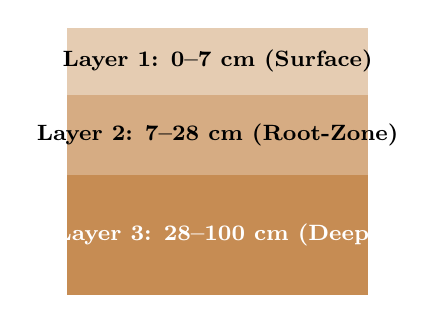
\begin{tikzpicture}[scale=0.85]
                    \fill[brown!40] (0, 3) rectangle (4.5, 4);
                    \node at (2.25, 3.5) {\footnotesize \textbf{Layer 1: 0--7 cm (Surface)}};
                    
                    \fill[brown!65] (0, 1.8) rectangle (4.5, 3);
                    \node at (2.25, 2.4) {\footnotesize \textbf{Layer 2: 7--28 cm (Root-Zone)}};
                    
                    \fill[brown!90] (0, 0) rectangle (4.5, 1.8);
                    \node at (2.25, 0.9) {\footnotesize \color{white}\textbf{Layer 3: 28--100 cm (Deep)}};
                \end{tikzpicture}
                \vspace{0.1cm}
                \footnotesize
                \textit{Each depth layer exhibits distinct hydrological response times and vertical percolation delays.}
            \end{exampleblock}
        \end{column}
    \end{columns}
\end{frame}

% ── Slide 4: Study Area: Mangaluru ────────────────────────────────────
\begin{frame}{Study Site: Mangaluru, Coastal Karnataka}
    \begin{columns}
        \begin{column}{0.50\textwidth}
            \begin{block}{\textbf{Site Coordinates \& Climate Context}}
                \footnotesize
                \begin{itemize}
                    \item \textbf{Location}: $12.9141^\circ\text{ N}, 74.8560^\circ\text{ E}$ (Dakshina Kannada).
                    \item \textbf{Climate}: Tropical Monsoon (Köppen \textit{Am}).
                    \item \textbf{Annual Rainfall}: 3,500--4,000 mm ($>85\%$ in June--Sept).
                \end{itemize}
            \end{block}
            \vspace{0.15cm}
            \begin{alertblock}{\textbf{Why is this an Ideal Testbed?}}
                \footnotesize
                \begin{itemize}
                    \item \textbf{Extreme swings}: Near-saturation ($>0.35$) in monsoon to desiccation ($<0.05\text{ m}^3/\text{m}^3$) in dry season.
                    \item Rigorously evaluates ML generalization under extreme precipitation events ($>25\text{ mm/day}$).
                \end{itemize}
            \end{alertblock}
        \end{column}
        \begin{column}{0.48\textwidth}
            \begin{exampleblock}{\textbf{Atmospheric \& Soil Drivers}}
                \centering
                \footnotesize
                \begin{tabular}{lc}
                    \toprule
                    \textbf{Environmental Driver} & \textbf{Typical Range} \\
                    \midrule
                    Daily Mean Temp ($T_{\text{mean}}$) & 24 -- 32 $^\circ\text{C}$ \\
                    Relative Humidity ($RH_{\text{mean}}$) & 65 -- 95 \% \\
                    Peak Monsoonal Rain & $>100\text{ mm/day}$ \\
                    Surface SM ($0\text{--}7\text{ cm}$) & 0.04 -- 0.38 $\text{m}^3/\text{m}^3$ \\
                    Deep SM ($28\text{--}100\text{ cm}$) & 0.06 -- 0.25 $\text{m}^3/\text{m}^3$ \\
                    \bottomrule
                \end{tabular}
            \end{exampleblock}
        \end{column}
    \end{columns}
\end{frame}

% ── Slide 4b: Multi-Site Study Areas in Karnataka ─────────────────────
\begin{frame}{Study Areas: Coastal, Plateau, and Western Ghats Regimes}
    \begin{columns}
        \begin{column}{0.48\textwidth}
            \centering
            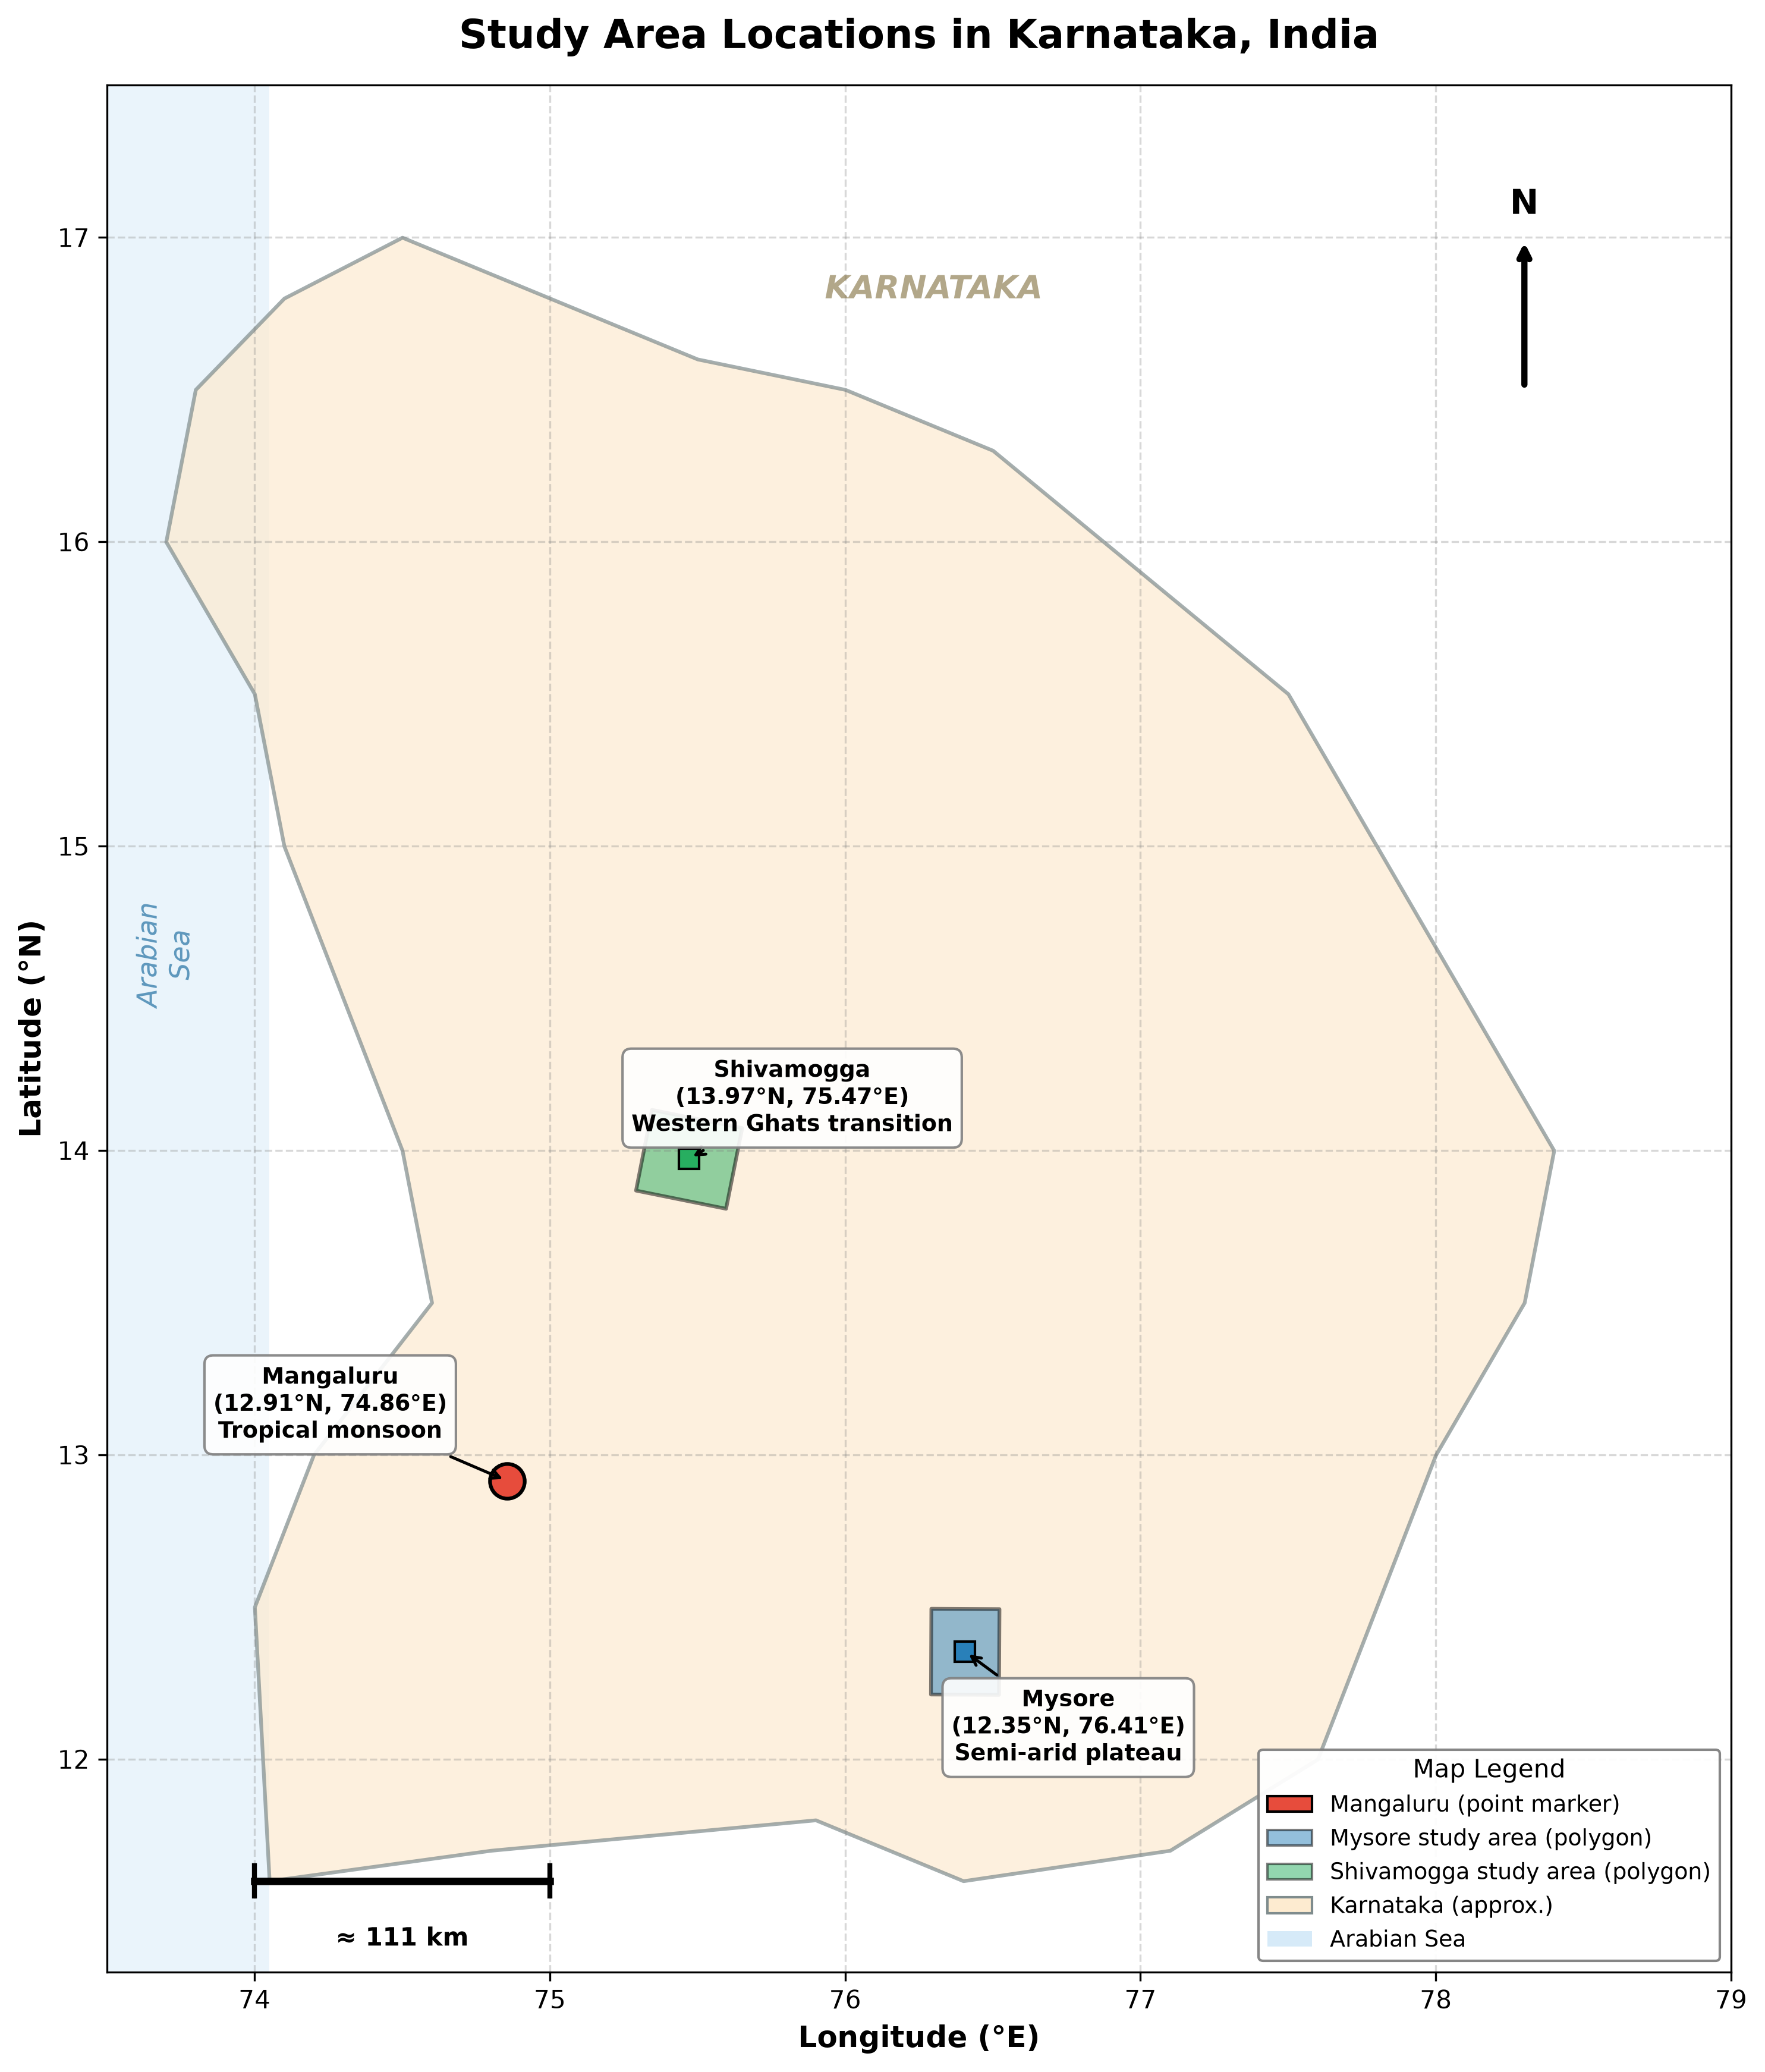
\includegraphics[width=0.92\textwidth]{figures/fig_study_area_map.png}
        \end{column}
        \begin{column}{0.50\textwidth}
            \begin{block}{\textbf{Three Distinct Agro-Climatic Regimes}}
                \footnotesize
                \begin{itemize}
                    \item \textbf{Mangaluru} (Coastal Lowland, $12.91^\circ\text{N}$):
                    \begin{itemize}
                        \item Annual rain: $3,510\text{ mm}$ (Köppen \textit{Am}).
                        \item Massive monsoonal wetting and steep dry-down.
                    \end{itemize}
                    \item \textbf{Mysore} (Southern Deccan Plateau, $12.35^\circ\text{N}$):
                    \begin{itemize}
                        \item Leeward rain-shadow, annual rain: $1,087\text{ mm}$ (\textit{BSh}).
                        \item Semi-arid regime with high evaporative demand.
                    \end{itemize}
                    \item \textbf{Shivamogga} (Ghats Transition, $13.97^\circ\text{N}$):
                    \begin{itemize}
                        \item Malnad transitional zone, annual rain: $1,162\text{ mm}$ (\textit{Aw}).
                        \item Intensive paddy and plantation agriculture.
                    \end{itemize}
                \end{itemize}
            \end{block}
        \end{column}
    \end{columns}
\end{frame}

% ── Slide 5: Reference Paper & Our Extensions ─────────────────────────
\begin{frame}{Reference Paper vs.\ Our Extensions}
    \begin{block}{\textbf{Baseline: Gao et al.\ (2026), \textit{Smart Agricultural Technology}}}
        \footnotesize
        Proposed recursive multi-step surface forecasting with gradient boosting and sequential deep-layer estimation from meteorological variables.
    \end{block}

    \vspace{0.1cm}
    \begin{columns}[t]
        \begin{column}{0.48\textwidth}
            \begin{exampleblock}{\textbf{1. Training on Real Weather Forecasts}}
                \footnotesize
                Baseline assumes perfect future weather. We train directly on \textbf{ECMWF operational forecasts} (lead 1--7), making the model resilient to weather errors.
            \end{exampleblock}
            \vspace{0.1cm}
            \begin{exampleblock}{\textbf{2. Long-Memory Hydrological Features}}
                \footnotesize
                Deep soil responds over weeks. We engineered rolling 7, 14, and 30-day cumulative rainfall and memory to capture vertical percolation.
            \end{exampleblock}
        \end{column}
        \begin{column}{0.48\textwidth}
            \begin{exampleblock}{\textbf{3. Strict Chronological Evaluation}}
                \footnotesize
                Random splits leak temporal autocorrelation. We prove random splits artificially inflate deep-layer scores by up to $50\%$ and enforce strict time splits.
            \end{exampleblock}
            \vspace{0.1cm}
            \begin{exampleblock}{\textbf{4. Satellite Radar Feasibility Study}}
                \footnotesize
                Integrated Sentinel-1 SAR and Sentinel-2 NDVI via Google Earth Engine to benchmark radar retrieval against reanalysis.
            \end{exampleblock}
        \end{column}
    \end{columns}
\end{frame}

% ── Slide 6: Multi-Source Data Architecture ───────────────────────────
\begin{frame}{Multi-Source Data Architecture \& Preprocessing}
    \begin{columns}[t]
        \begin{column}{0.32\textwidth}
            \begin{block}{\textbf{ERA5-Land Target}}
                \footnotesize
                \begin{itemize}
                    \item 3-year hourly record (2023--2025).
                    \item Volumetric water content for 3 target depths ($0\text{--}7$, $7\text{--}28$, $28\text{--}100\text{ cm}$).
                    \item Daily surface pressure, wind speed, solar forcing.
                \end{itemize}
            \end{block}
        \end{column}
        \begin{column}{0.34\textwidth}
            \begin{block}{\textbf{ECMWF Forecasts}}
                \footnotesize
                \begin{itemize}
                    \item Archived operational IFS 0.25$^\circ$ model runs.
                    \item Leads 1 to 7 days ahead for target dates.
                    \item Daily $T_{\max}$, $T_{\min}$, $RH_{\text{mean}}$, and total precipitation.
                \end{itemize}
            \end{block}
        \end{column}
        \begin{column}{0.32\textwidth}
            \begin{block}{\textbf{Satellite Data}}
                \footnotesize
                \begin{itemize}
                    \item \textbf{Sentinel-1 GRD}: C-band SAR backscatter (VV, VH, RVI).
                    \item \textbf{Sentinel-2 MSI}: Cloud-masked optical NDVI for vegetation density.
                    \item 150 m spatial buffer.
                \end{itemize}
            \end{block}
        \end{column}
    \end{columns}

    \vspace{0.25cm}
    \begin{exampleblock}{\textbf{Feature Engineering Engine (Physics-Inspired Inputs)}}
        \footnotesize
        \begin{itemize}
            \item \textbf{Autoregressive Surface Memory}: $SM_{t-1}, SM_{t-2}$ captures prior capillary retention.
            \item \textbf{Atmospheric Evaporative Demand}: Diurnal range $T_{\text{range}} = T_{\max} - T_{\min}$, relative humidity $RH$.
            \item \textbf{Long-Memory Rolling Windows}: Cumulative rainfall ($\text{Rain}_{7d}, \text{Rain}_{14d}, \text{Rain}_{30d}$) and rolling mean soil moisture ($SM_{\text{mean}7}, SM_{\text{mean}30}$) capture gradual downward percolation into deeper profiles.
        \end{itemize}
    \end{exampleblock}
\end{frame}

% ── Slide 7: Methodology: Progressive Chaining ────────────────────────
\begin{frame}{System Pipeline: Progressive Chaining Architecture}
    \begin{columns}
        \begin{column}{0.58\textwidth}
            \begin{block}{\textbf{Physics-Inspired Staged Prediction}}
                \footnotesize
                Rather than predicting all depths independently, we mirror downward gravity-driven percolation:
                \vspace{0.15cm}
                \begin{enumerate}
                    \item \textbf{Stage 1: Recursive Surface Forecasting ($0\text{--}7\text{ cm}$)}
                    \vspace{0.05cm}
                    $$\widehat{SM}_{t+k}^{(0\text{--}7)} = f_{\text{XGB}}\left(\widehat{SM}_{t+k-1}, \widehat{SM}_{t+k-2}, \mathbf{W}_{t+k}^{\text{fc}}, k\right)$$
                    \item \textbf{Stage 2: Intermediate Root-Zone ($7\text{--}28\text{ cm}$)}
                    \vspace{0.05cm}
                    $$\widehat{SM}_{t}^{(7\text{--}28)} = g_{\text{XGB}}\left(\widehat{SM}_{t}^{(0\text{--}7)}, \mathbf{W}_{t}, \text{LongMemory}_{t}\right)$$
                    \item \textbf{Stage 3: Deep Root-Zone ($28\text{--}100\text{ cm}$)}
                    \vspace{0.05cm}
                    $$\widehat{SM}_{t}^{(28\text{--}100)} = h_{\text{XGB}}\left(\widehat{SM}_{t}^{(0\text{--}7)}, \widehat{SM}_{t}^{(7\text{--}28)}, \mathbf{W}_{t}, \text{LongMemory}_{t}\right)$$
                \end{enumerate}
            \end{block}
        \end{column}
        \begin{column}{0.40\textwidth}
            \begin{exampleblock}{\textbf{Why Chaining Works}}
                \footnotesize
                \begin{itemize}
                    \item Deeper soil columns do not exchange moisture directly with the atmosphere; they respond to percolation through overlying layers.
                    \item By feeding $\widehat{SM}^{(7\text{--}28)}$ into Stage 3, the model enforces \textbf{vertical physical consistency}.
                    \item Completely replaces missing underground IoT telemetry with data-driven physical inference.
                \end{itemize}
            \end{exampleblock}
        \end{column}
    \end{columns}
\end{frame}

% ── Slide 8: Machine Learning Formulation: XGBoost ───────────────────
\begin{frame}{Why XGBoost for Hydrological Time-Series?}
    \begin{columns}
        \begin{column}{0.48\textwidth}
            \begin{block}{\textbf{Extreme Gradient Boosting (XGBoost)}}
                \begin{itemize}
                    \item Ensemble of decision trees trained sequentially to minimize residual loss:
                    $$\hat{y}_i = \sum_{m=1}^{M} f_m(\mathbf{x}_i)$$
                    \item \textbf{Non-linear thresholds}: Solves physical saturation limits (soil porosity saturation vs.\ field capacity vs.\ wilting point) naturally without manual piecewise equations.
                    \item \textbf{Built-in Regularization}: $L_1$ and $L_2$ penalties on leaf weights suppress overfitting during recursive error accumulation.
                \end{itemize}
            \end{block}
        \end{column}
        \begin{column}{0.48\textwidth}
            \begin{exampleblock}{\textbf{Optimized Model Hyperparameters}}
                \small
                \begin{tabular}{ll}
                    \toprule
                    \textbf{Parameter} & \textbf{Tuned Value} \\
                    \midrule
                    Base Estimator & Tree Regressor \\
                    Number of Trees ($M$) & 400 \\
                    Maximum Tree Depth & 3 (shallow to curb drift) \\
                    Learning Rate ($\eta$) & 0.05 \\
                    CV Scheme & 5-Fold TimeSeriesSplit \\
                    Loss Function & Root Mean Squared Error \\
                    \bottomrule
                \end{tabular}
                \vspace{0.15cm}
                \footnotesize
                \textit{A shallow depth ($max\_depth=3$) avoids overfitting to extreme single-day rainfall anomalies.}
            \end{exampleblock}
        \end{column}
    \end{columns}
\end{frame}

% ── Slide 9: Finding 1: Train/Test Split Leakage ───────────────────────
\begin{frame}{Key Finding 1: The Peril of Random Train/Test Splitting}
    \begin{columns}
        \begin{column}{0.45\textwidth}
            \begin{alertblock}{\textbf{Temporal Autocorrelation Leakage}}
                \footnotesize
                \begin{itemize}
                    \item Soil moisture changes gradually from day to day.
                    \item When days are randomly shuffled, day $t-1$ and $t+1$ land in training while day $t$ is in test.
                    \item The model merely interpolates adjacent points, producing deceptively high scores ($R^2 > 0.70$ on deep layers).
                    \item Under strict \textbf{chronological split}, real generalization drops sharply ($R^2 = 0.35$ for baseline).
                \end{itemize}
            \end{alertblock}
        \end{column}
        \begin{column}{0.53\textwidth}
            \centering
            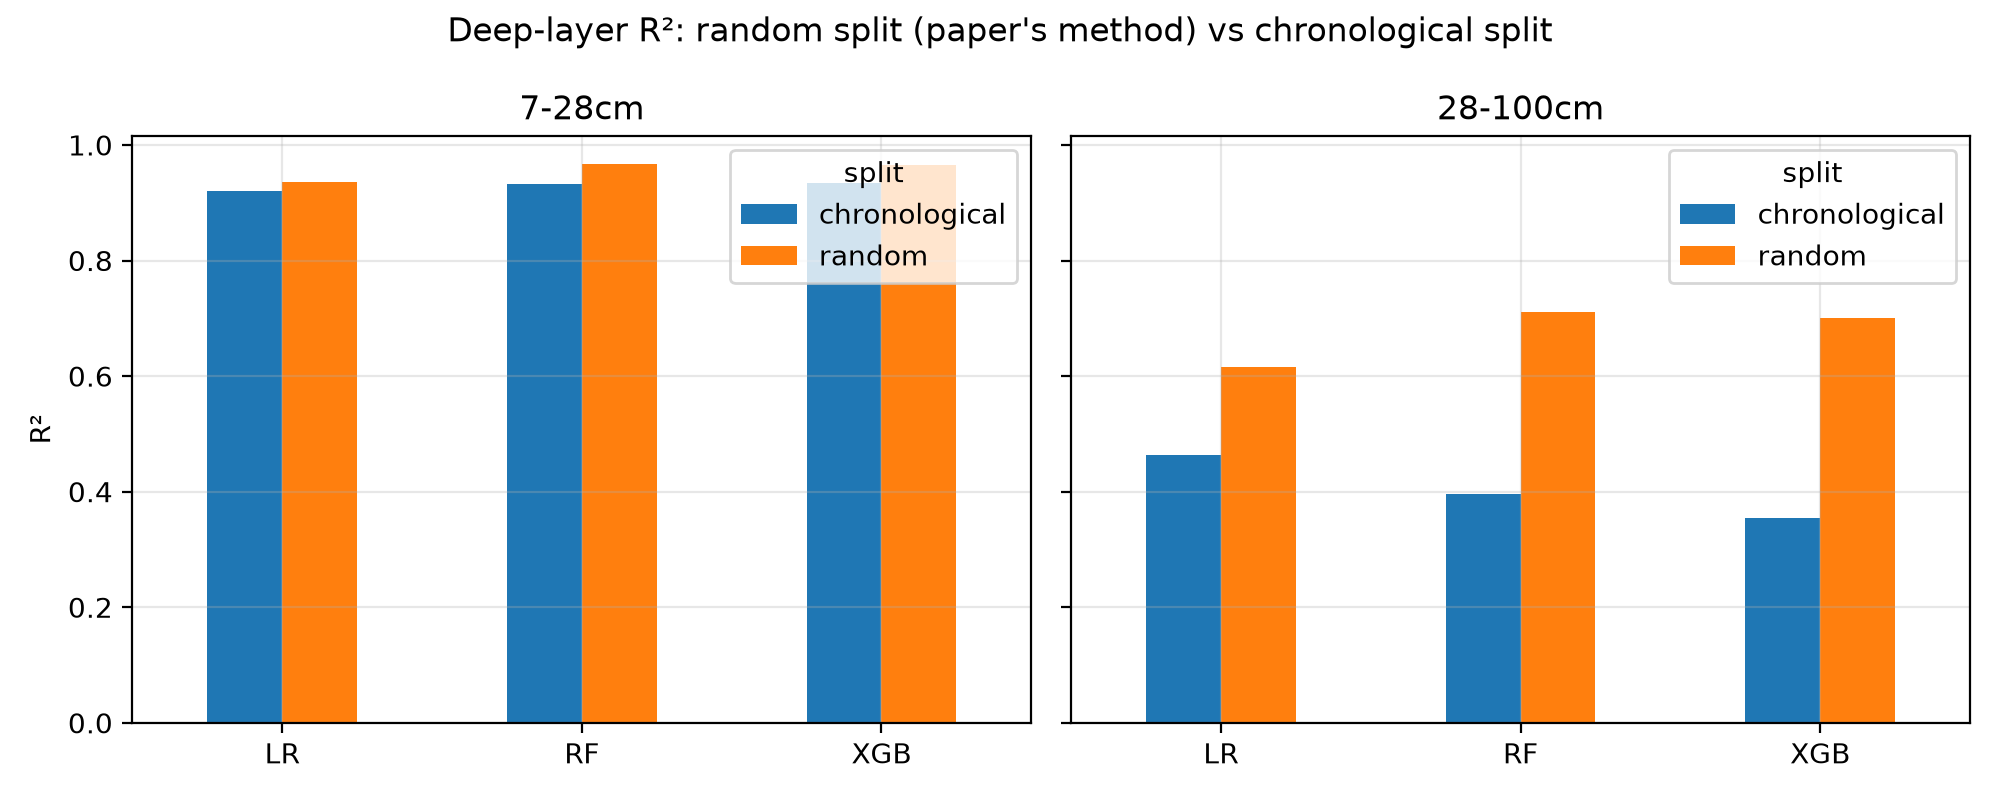
\includegraphics[width=\textwidth]{figures/fig2_split_comparison.png}\\
            \vspace{0.1cm}
            \footnotesize \textit{Comparison of test $R^2$: Random Split (paper's method) vs.\ Chronological Split.}
        \end{column}
    \end{columns}
\end{frame}

% ── Slide 10: Finding 2: Surface Forecast Horizon ─────────────────────
\begin{frame}{Key Finding 2: 7-Day Out-of-Sample Surface Forecast}
    \begin{columns}
        \begin{column}{0.50\textwidth}
            \centering
            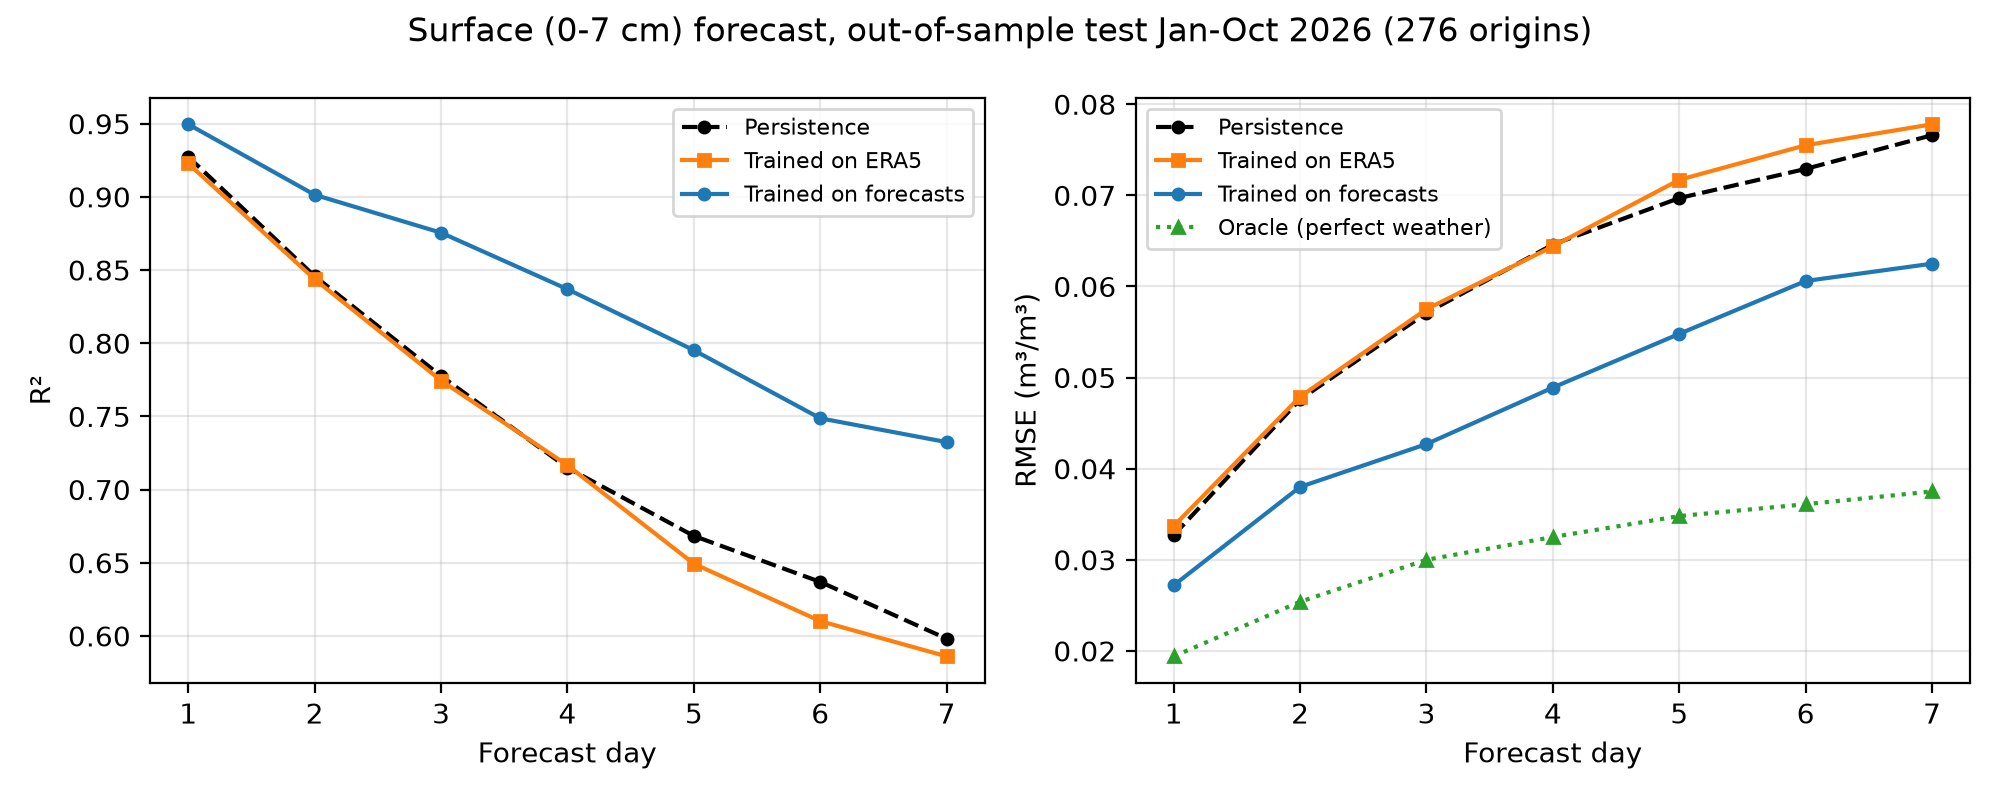
\includegraphics[width=\textwidth]{figures/fig1_forecast_horizon.png}
        \end{column}
        \begin{column}{0.48\textwidth}
            \begin{block}{\textbf{Performance on 2026 Test (276 Forecasts)}}
                \footnotesize
                \begin{itemize}
                    \item \textbf{Trained on Forecasts (Ours)}:
                    \begin{itemize}
                        \item Day 1: $R^2 = \mathbf{0.950}$, $\text{RMSE} = \mathbf{0.027}\text{ m}^3/\text{m}^3$
                        \item Day 7: $R^2 = \mathbf{0.732}$, $\text{RMSE} = \mathbf{0.063}\text{ m}^3/\text{m}^3$
                    \end{itemize}
                    \item \textbf{Persistence Baseline}:
                    \begin{itemize}
                        \item Day 1: $R^2 = 0.927$ \quad $\bullet$ \quad Day 7: $R^2 = 0.598$
                    \end{itemize}
                    \item \textbf{Trained on ERA5 (Paper's Method)}:
                    \begin{itemize}
                        \item Degrades to $R^2 = 0.586$ at Day 7 due to train/test weather distribution mismatch!
                    \end{itemize}
                \end{itemize}
            \end{block}
            \vspace{0.05cm}
            \footnotesize \textbf{Takeaway}: Lead-time conditioning and forecast training preserve predictive skill.
        \end{column}
    \end{columns}
\end{frame}

% ── Slide 11: Finding 3: Weather Forecast Robustness ──────────────────
\begin{frame}{Key Finding 3: Stress-Testing Weather Uncertainty}
    \begin{columns}
        \begin{column}{0.48\textwidth}
            \begin{block}{\textbf{Simulated Numerical Weather Errors}}
                \footnotesize
                We perturbed future meteorological inputs to test operational breakdown points:
                \begin{itemize}
                    \item \textbf{Oracle (Perfect Weather)}: Day-7 $R^2 = \mathbf{0.938}$
                    \item \textbf{Mild Noise} ($\sigma_T=1^\circ\text{C}, \sigma_{\text{rain}}=50\%$): Day-7 $R^2 = \mathbf{0.895}$
                    \item \textbf{Heavy Noise} ($\sigma_T=2^\circ\text{C}, \sigma_{\text{rain}}=100\%$): Day-7 $R^2 = \mathbf{0.794}$
                    \item \textbf{No Forecast (Climatology)}: Day-7 $R^2 = 0.439$ (fails!)
                    \item \textbf{Persistence Baseline}: Day-7 $R^2 = 0.575$
                \end{itemize}
            \end{block}
        \end{column}
        \begin{column}{0.48\textwidth}
            \begin{exampleblock}{\textbf{Monsoon vs.\ Dry Season Skill}}
                \footnotesize
                \centering
                \begin{tabular}{lccc}
                    \toprule
                    \textbf{Season} & \textbf{Day 1} & \textbf{Day 3} & \textbf{Day 7} \\
                    \midrule
                    \textit{Dry/Pre-Monsoon} & 0.034 & 0.054 & 0.074 \\
                    \textit{Monsoon (Jun--Sep)} & \textbf{0.033} & 0.062 & 0.083 \\
                    \bottomrule
                \end{tabular}
                \vspace{0.2cm}
                \flushleft
                \begin{itemize}
                    \item Monsoon heavy rainfall events ($\ge 25\text{ mm/day}$, $n=33$ days in 2026) increase day-7 variance.
                    \item However, ML model remains substantially superior to persistence under all noise regimes.
                \end{itemize}
            \end{exampleblock}
        \end{column}
    \end{columns}
\end{frame}

% ── Slide 12: Finding 4: Long-Memory Feature Engineering ──────────────
\begin{frame}{Key Finding 4: Power of Long-Memory Features}
    \begin{columns}
        \begin{column}{0.46\textwidth}
            \begin{block}{\textbf{Why Daily Weather Fails for Deep Layers}}
                \footnotesize
                \begin{itemize}
                    \item Subsurface soil ($28\text{--}100\text{ cm}$) has high thermal and hydraulic inertia.
                    \item A single rain event on day $t$ barely alters moisture at 80 cm depth on the same day.
                    \item Deep layers depend on the cumulative hydrological balance over the preceding weeks.
                    \item Introducing \textbf{rolling 7, 14, and 30-day precipitation and mean moisture} enables the model to resolve percolation delays.
                \end{itemize}
            \end{block}
        \end{column}
        \begin{column}{0.52\textwidth}
            \centering
            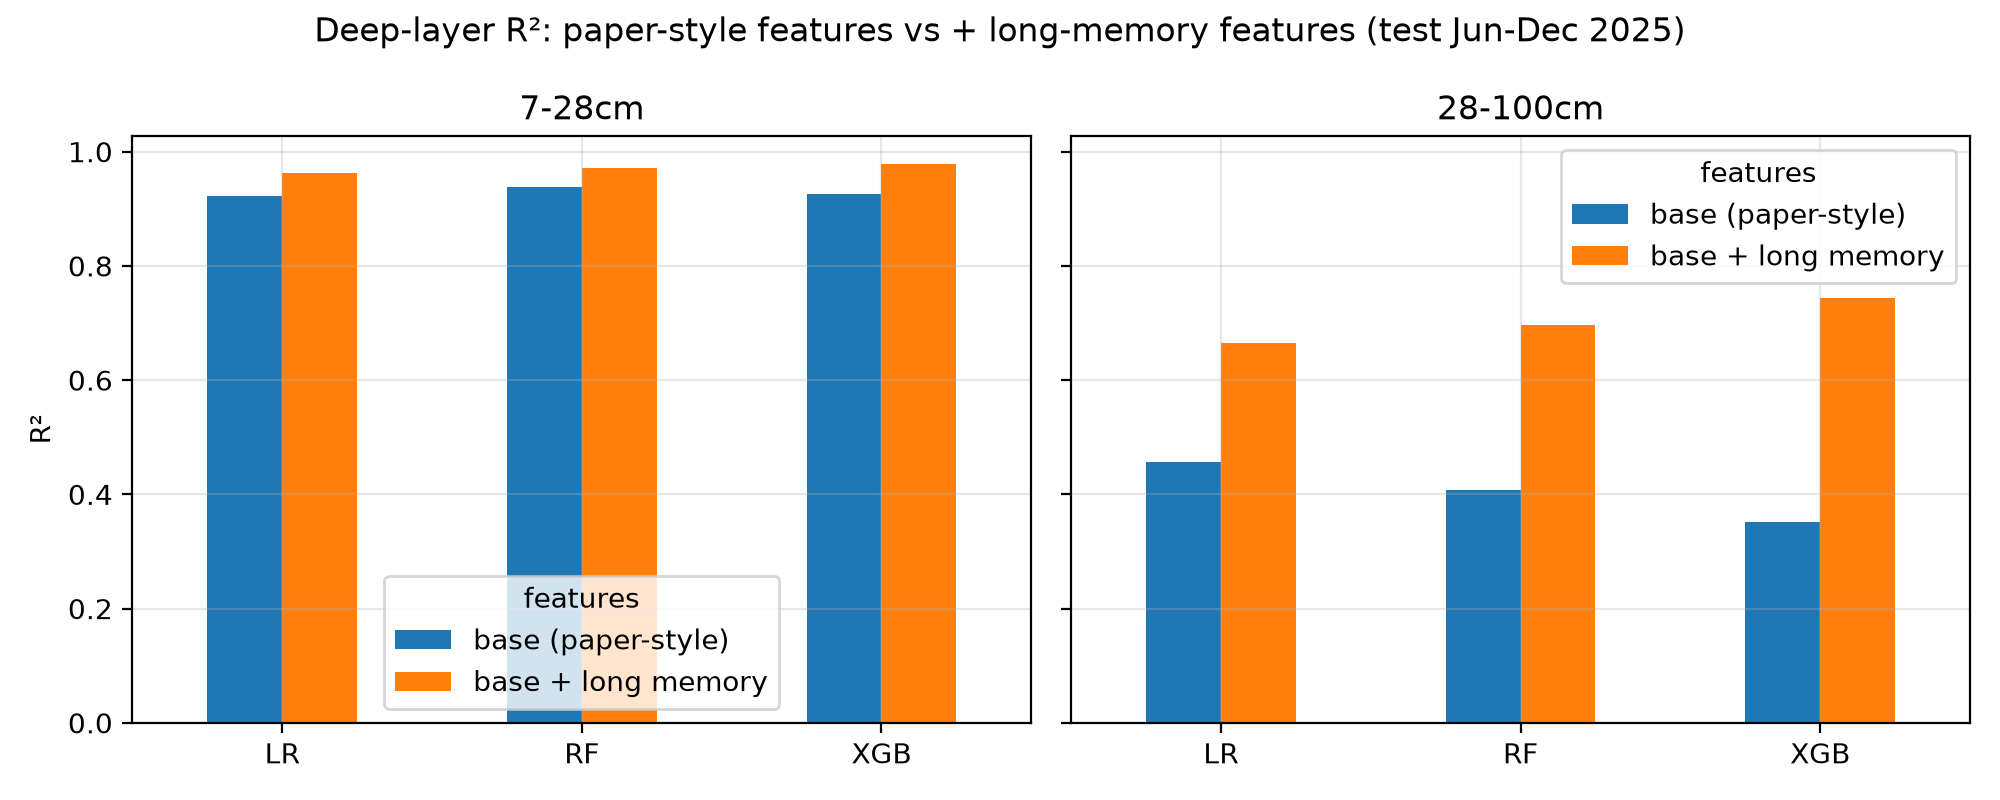
\includegraphics[width=\textwidth]{figures/fig3_long_memory.png}\\
            \vspace{0.1cm}
            \footnotesize \textit{$R^2$ jumps from $\mathbf{0.352} \rightarrow \mathbf{0.744}$ for 28--100 cm depth with long-memory features!}
        \end{column}
    \end{columns}
\end{frame}

% ── Slide 13: Finding 5: 2026 Deep-Layer Tracking ─────────────────────
\begin{frame}{Key Finding 5: Full 2026 Deep-Layer Out-of-Sample Backtest}
    \begin{columns}
        \begin{column}{0.52\textwidth}
            \centering
            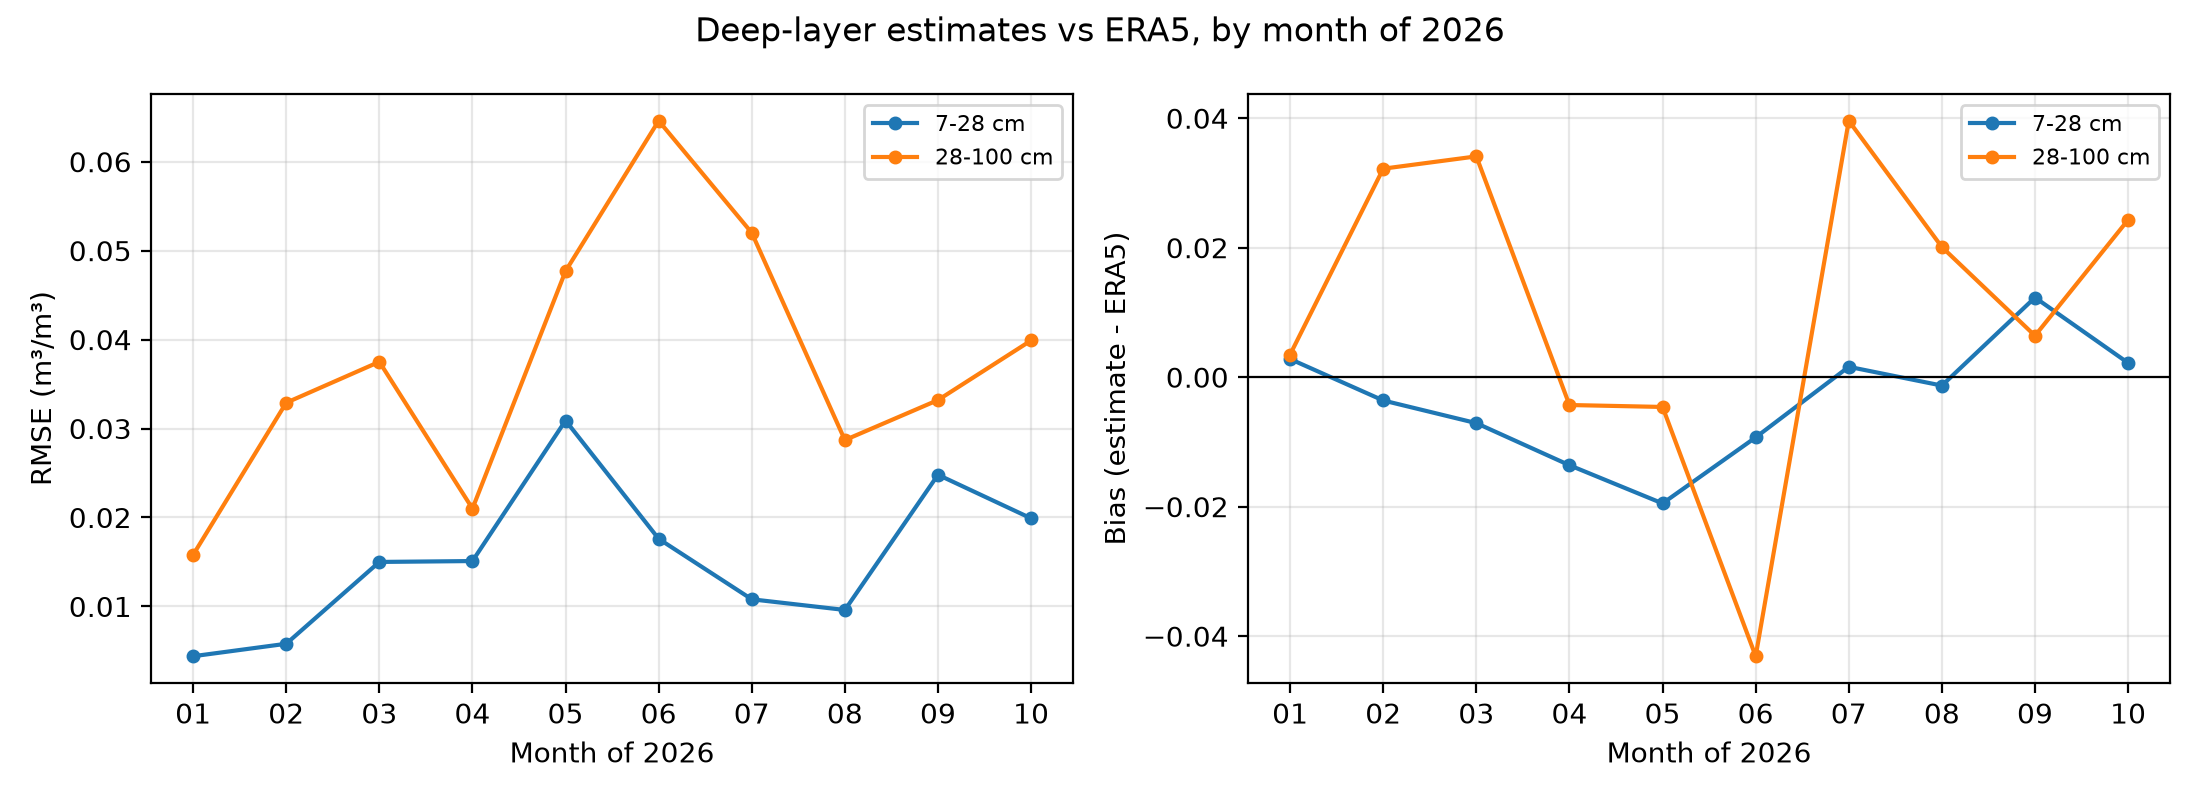
\includegraphics[width=\textwidth]{figures/fig4_deep_2026_monthly.png}
        \end{column}
        \begin{column}{0.45\textwidth}
            \begin{block}{\textbf{2026 Backtest Performance}}
                \footnotesize
                Models trained strictly up to Dec 2025:
                \begin{itemize}
                    \item \textbf{7--28 cm Layer}:
                    \begin{itemize}
                        \item $R^2 = \mathbf{0.975}$, $\text{RMSE} = \mathbf{0.017}\text{ m}^3/\text{m}^3$
                        \item $\text{Bias} = -0.0037$ (near zero!)
                        \item Tracks seasonal cycle and drying curves exceptionally well.
                    \end{itemize}
                    \item \textbf{28--100 cm Layer}:
                    \begin{itemize}
                        \item $R^2 = \mathbf{0.804}$, $\text{RMSE} = \mathbf{0.040}\text{ m}^3/\text{m}^3$
                        \item Mild positive bias ($+0.0105$).
                        \item Reliable for macro-reservoir tracking and water budget modeling.
                    \end{itemize}
                \end{itemize}
            \end{block}
        \end{column}
    \end{columns}
\end{frame}

% ── Slide 14: Finding 6: Satellite Radar Feasibility ──────────────────
\begin{frame}{Key Finding 6: Sentinel-1 Satellite Radar Feasibility}
    \begin{columns}
        \begin{column}{0.45\textwidth}
            \begin{block}{\textbf{The Satellite Remote Sensing Dilemma}}
                \footnotesize
                \begin{itemize}
                    \item Sentinel-1 SAR (C-band VV/VH) penetrates clouds during monsoon.
                    \item \textbf{Trap}: Raw radar models ($R^2 \approx 0.61\text{--}0.64$) perform \textit{worse} than simple monthly climatology ($R^2 = 0.725$)!
                    \item \textbf{Cause}: Annual vegetation growth cycle dominates backscatter, confusing radar soil dielectric response.
                    \item \textbf{Solution (Anomaly Model)}: Deseasonalize radar backscatter $\rightarrow$ predict moisture anomalies $\rightarrow$ $R^2$ jumps to $\mathbf{0.811}$!
                \end{itemize}
            \end{block}
        \end{column}
        \begin{column}{0.53\textwidth}
            \centering
            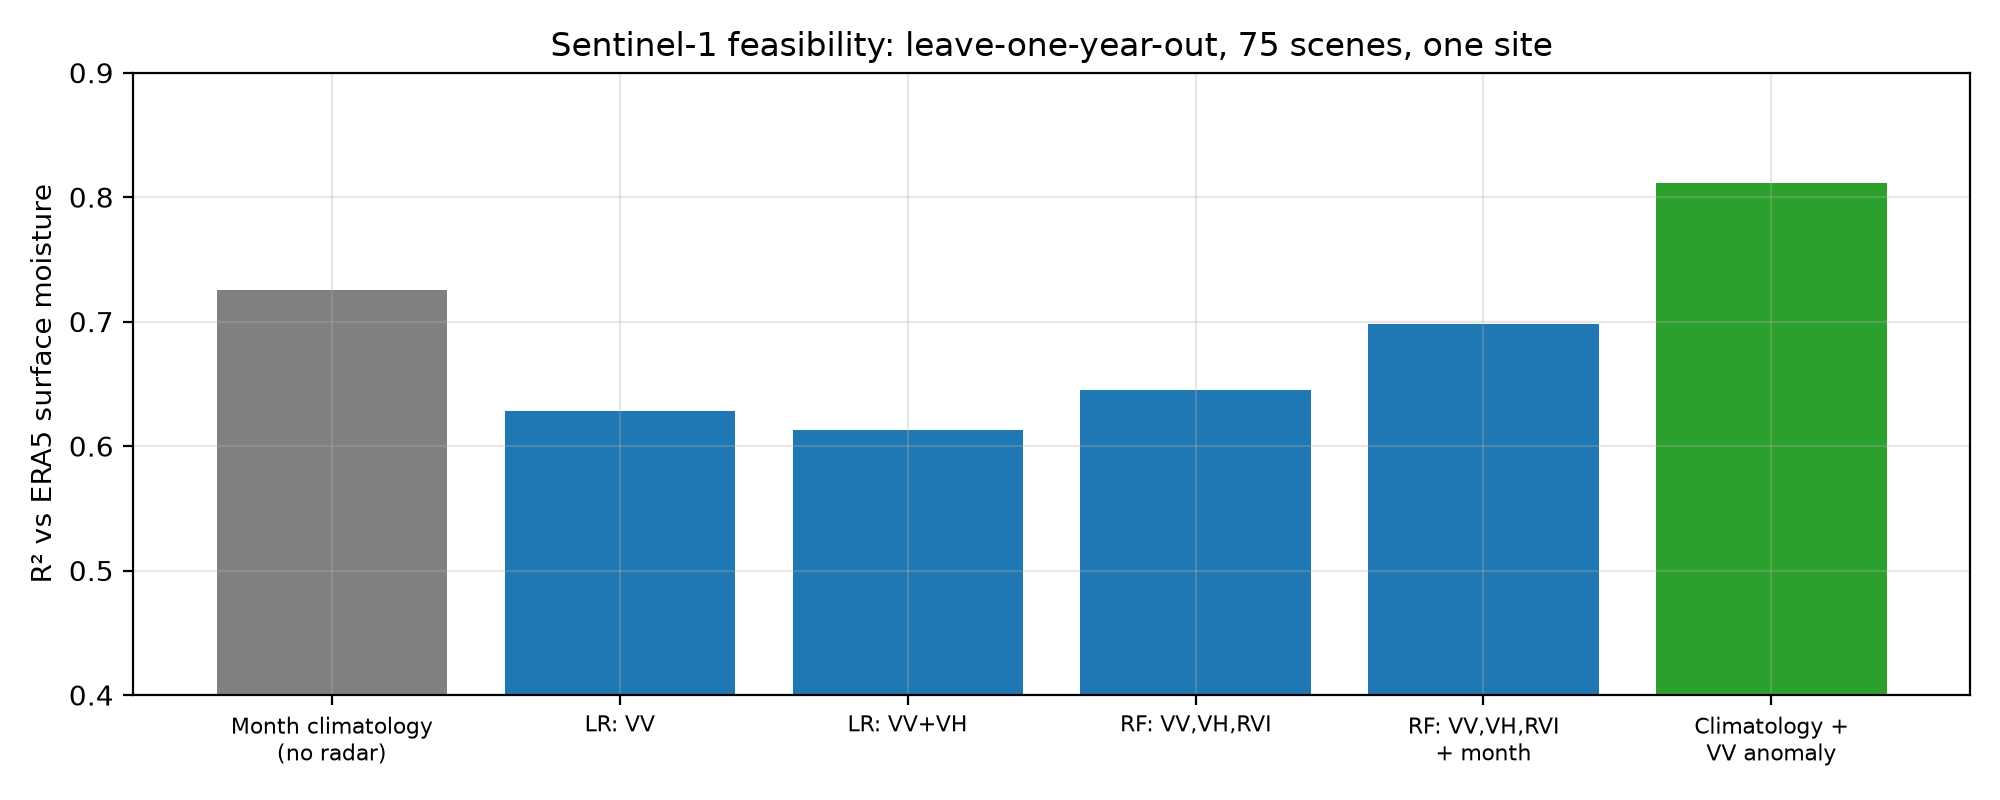
\includegraphics[width=\textwidth]{figures/fig5_satellite_feasibility.png}\\
            \vspace{0.1cm}
            \footnotesize \textit{Leave-One-Year-Out cross-validation across 75 Sentinel-1 scenes.}
        \end{column}
    \end{columns}
\end{frame}

% ── Slide 14b: Multi-Site Comparative Results ─────────────────────────
\begin{frame}{Key Finding 7: Multi-Site Cross-Regional Generalizability}
    \begin{columns}
        \begin{column}{0.50\textwidth}
            \centering
            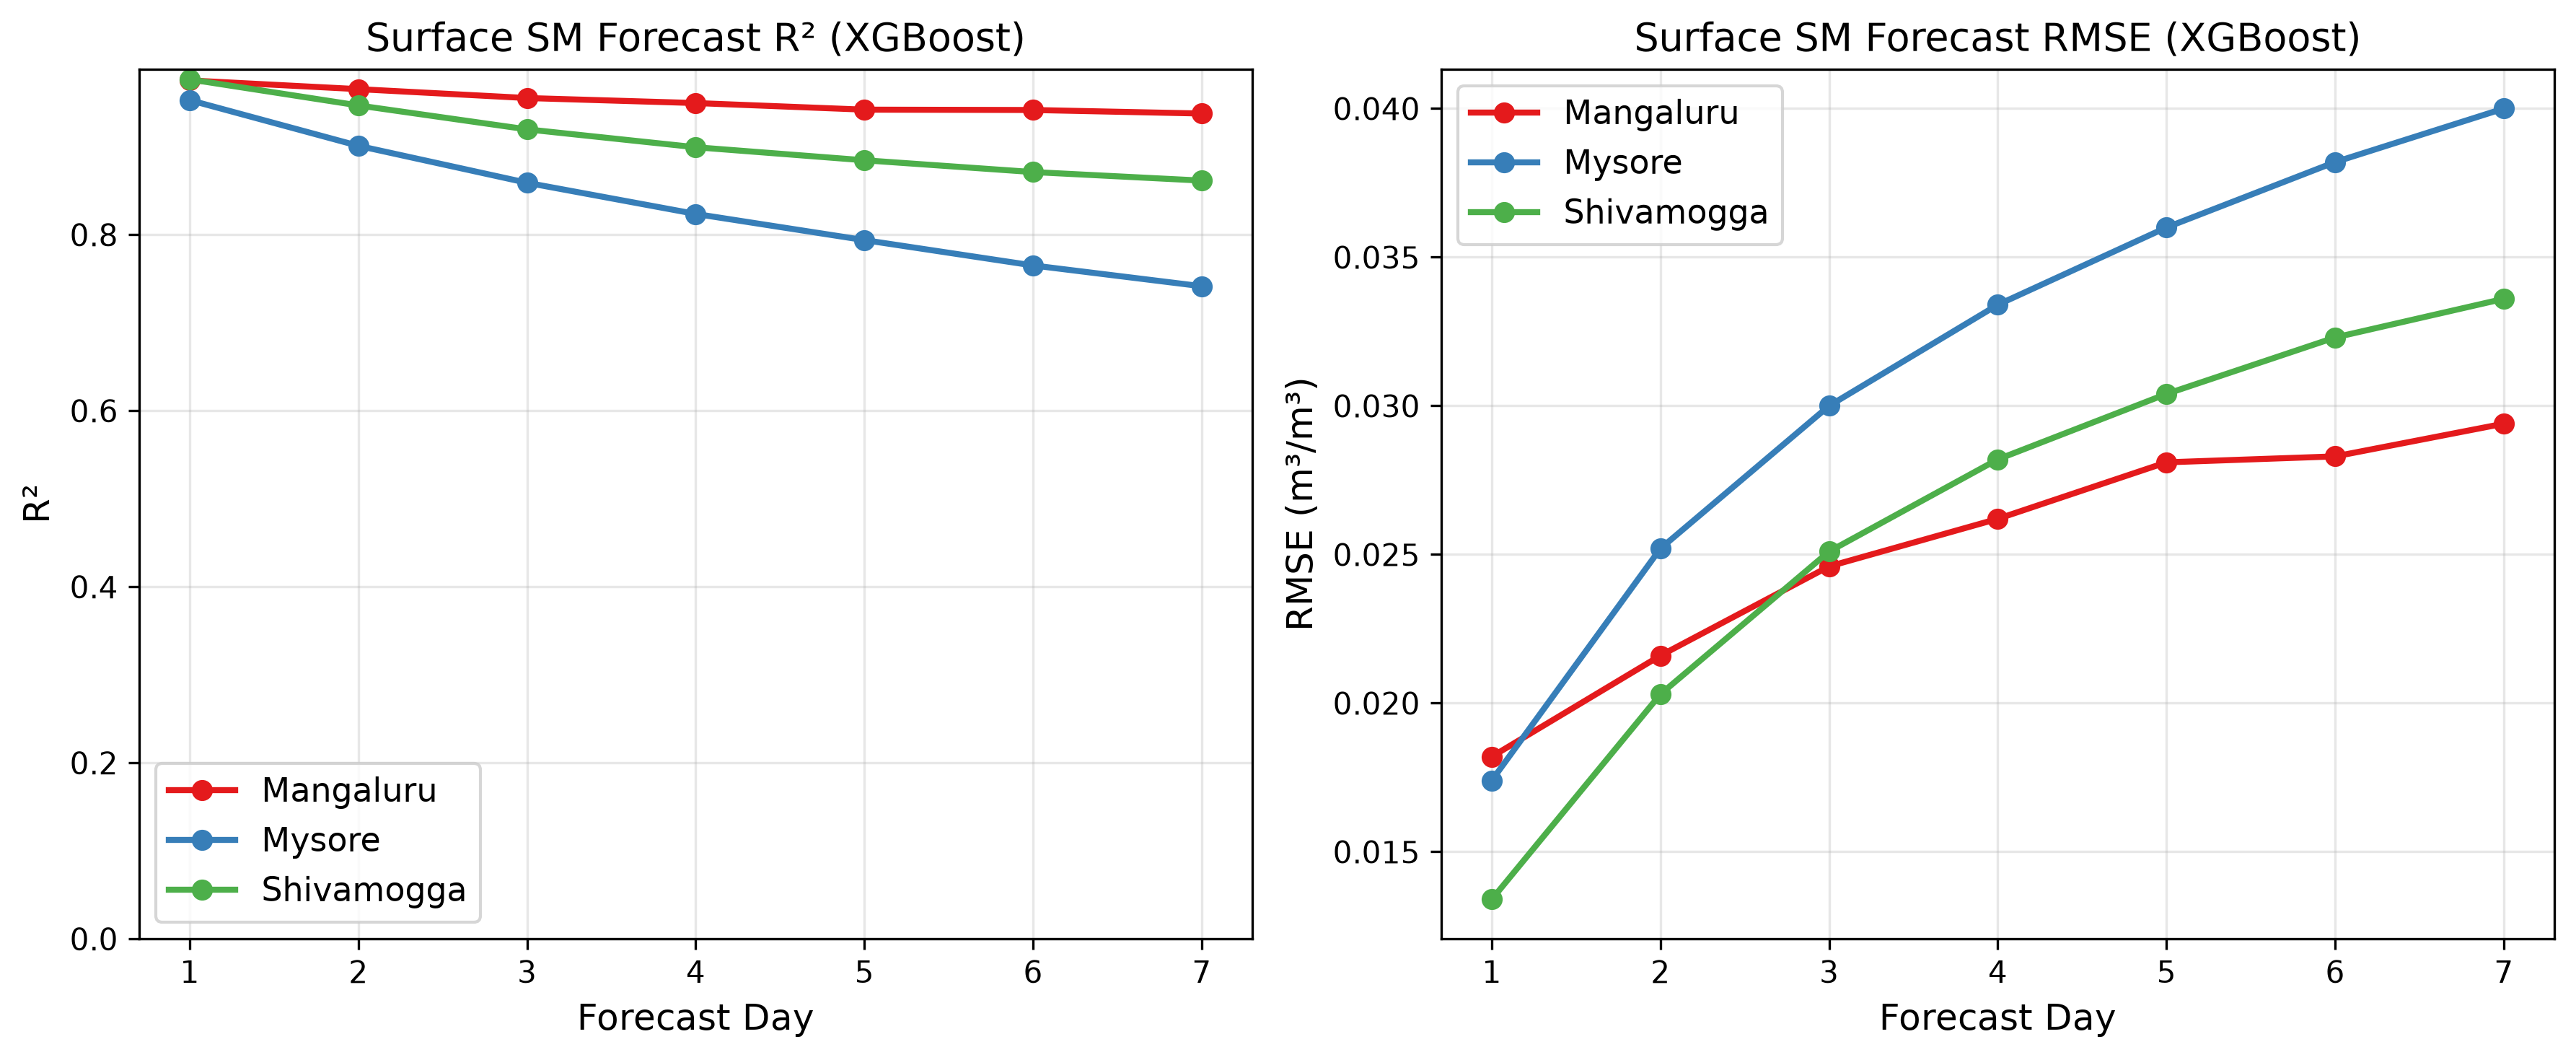
\includegraphics[width=\textwidth]{figures/fig6_cross_site_forecast.png}\\
            \vspace{0.05cm}
            \footnotesize \textit{Surface 7-day forecast skill across all three sites.}
        \end{column}
        \begin{column}{0.50\textwidth}
            \centering
            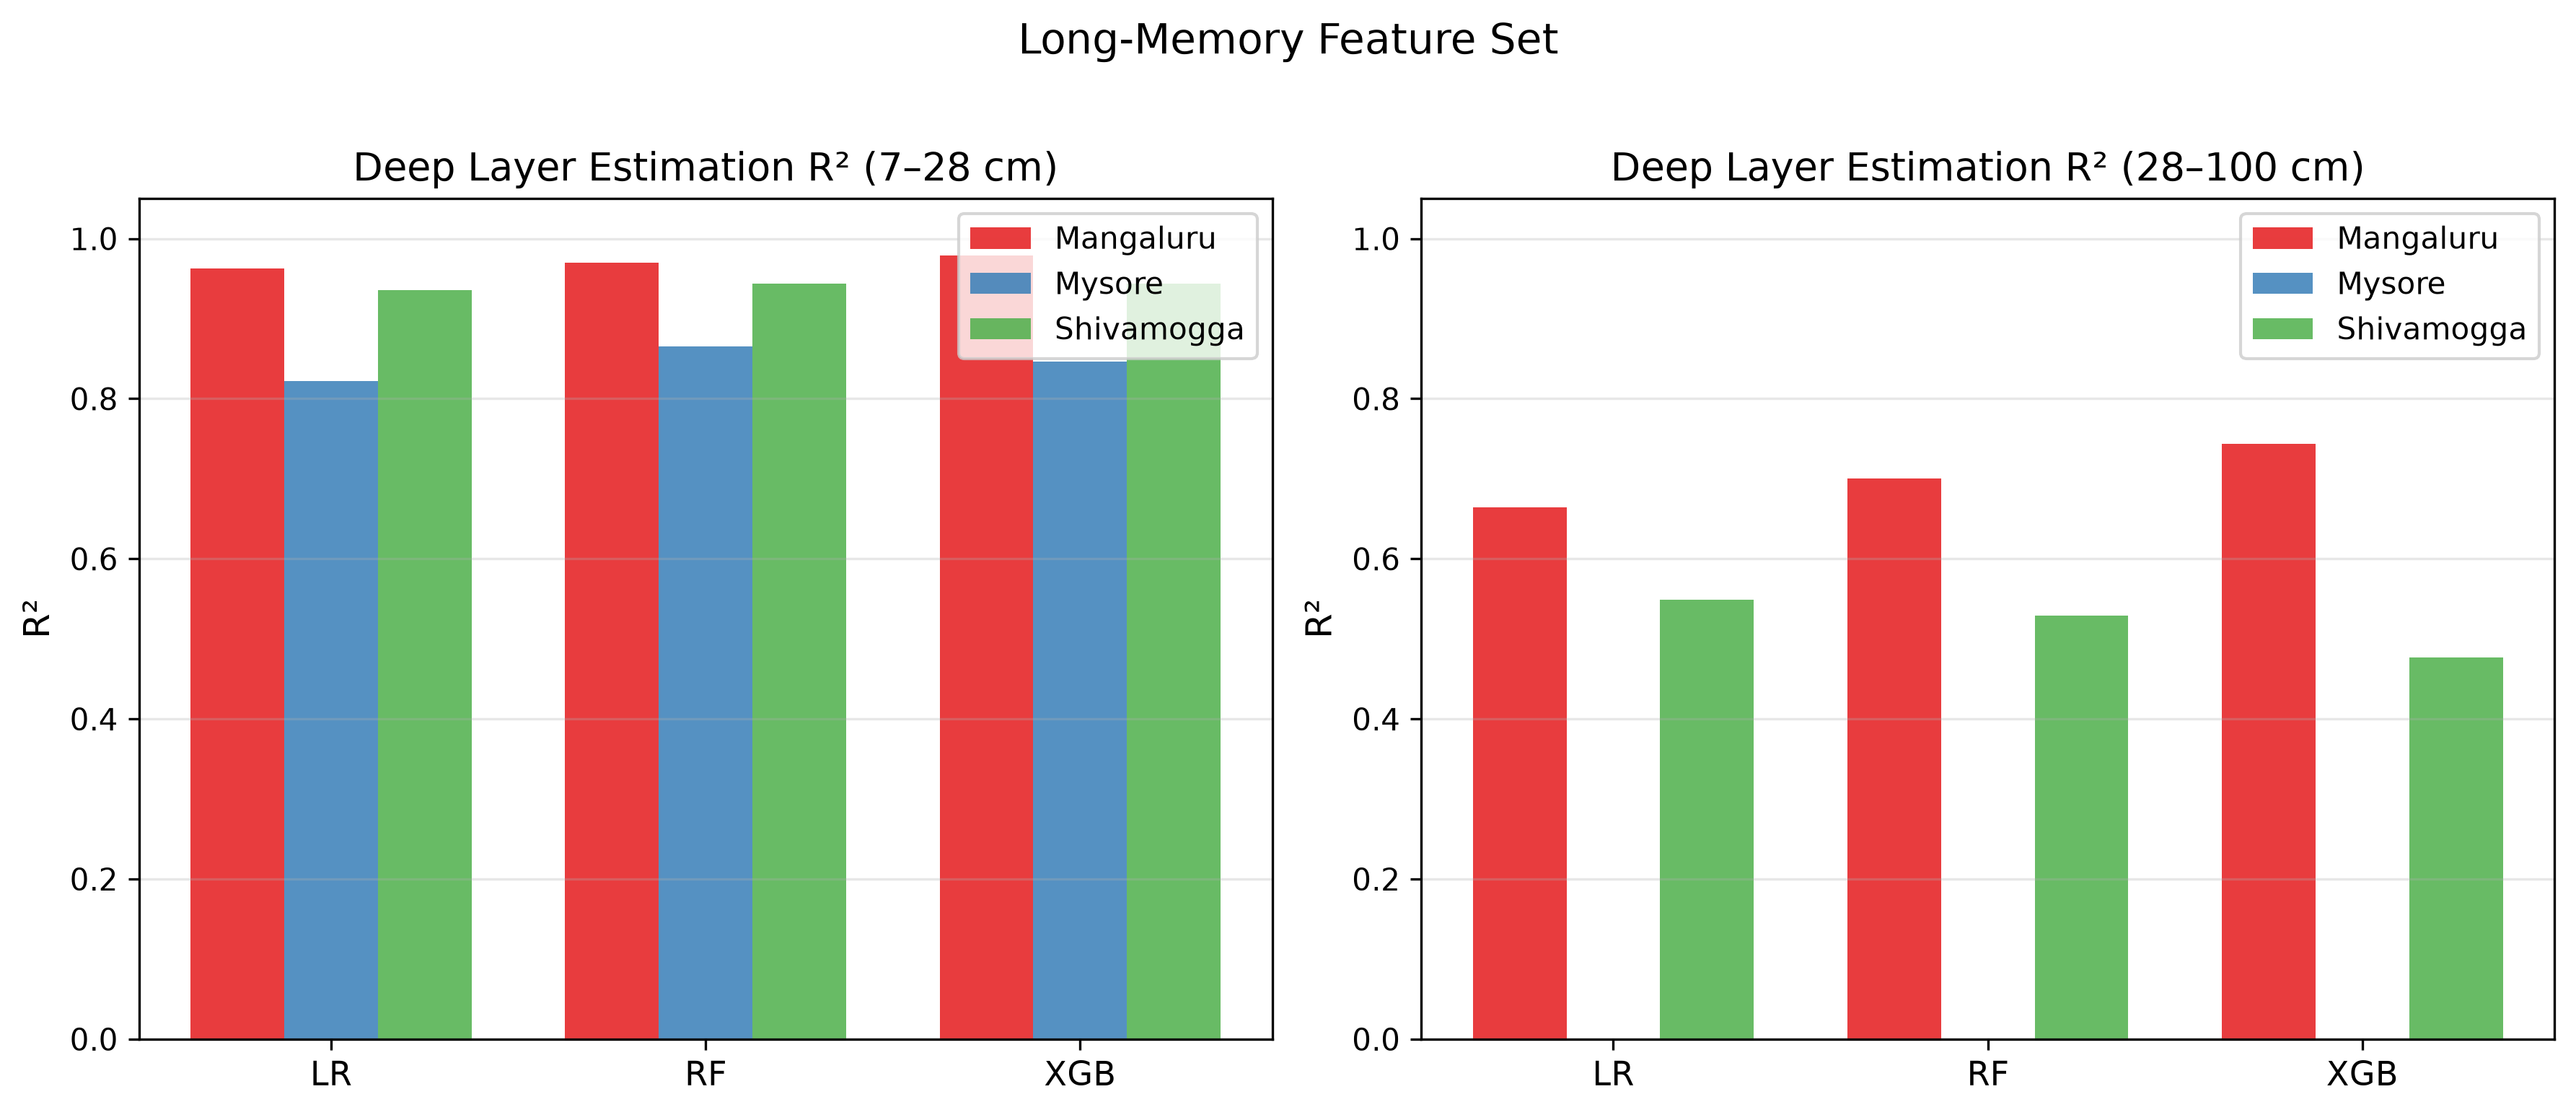
\includegraphics[width=\textwidth]{figures/fig7_cross_site_deep.png}\\
            \vspace{0.05cm}
            \footnotesize \textit{Deep-layer profile estimation across sites and algorithms.}
        \end{column}
    \end{columns}
    \vspace{0.15cm}
    \begin{alertblock}{\textbf{Cross-Regional Takeaways}}
        \footnotesize
        \begin{itemize}
            \item \textbf{Universal Forecast Superiority}: In semi-arid Mysore, persistence collapses to $R^2 = 0.22$ at Day 7, while XGBoost retains $R^2 = 0.74$!
            \item \textbf{High Stability}: Shivamogga achieves the lowest RMSE ($0.013\text{--}0.034\text{ m}^3/\text{m}^3$) across all 7 forecast days.
            \item \textbf{Deep Layer Percolation}: Long-memory features double deep $R^2$ in high-rainfall zones where percolation reaches 28--100 cm.
        \end{itemize}
    \end{alertblock}
\end{frame}

% ── Slide 15: Operational Dashboard ───────────────────────────────────
\begin{frame}{Operational Web Dashboard (Streamlit Prototype)}
    \begin{columns}
        \begin{column}{0.50\textwidth}
            \begin{block}{\textbf{Real-Time Pipeline (\texttt{app.py})}}
                \footnotesize
                \begin{enumerate}
                    \item \textbf{Automated Ingestion}: Queries Open-Meteo for the latest ERA5-Land records.
                    \item \textbf{Latency Bridging}: Forecasts the 2--5 day gap between last reanalysis and today.
                    \item \textbf{Recursive 7-Day Forecast}: Surface predictions with $\pm 1$ RMSE confidence.
                    \item \textbf{Chained Depth Profiling}: Progressive deep estimators replace subsurface probes.
                \end{enumerate}
            \end{block}
        \end{column}
        \begin{column}{0.48\textwidth}
            \centering
            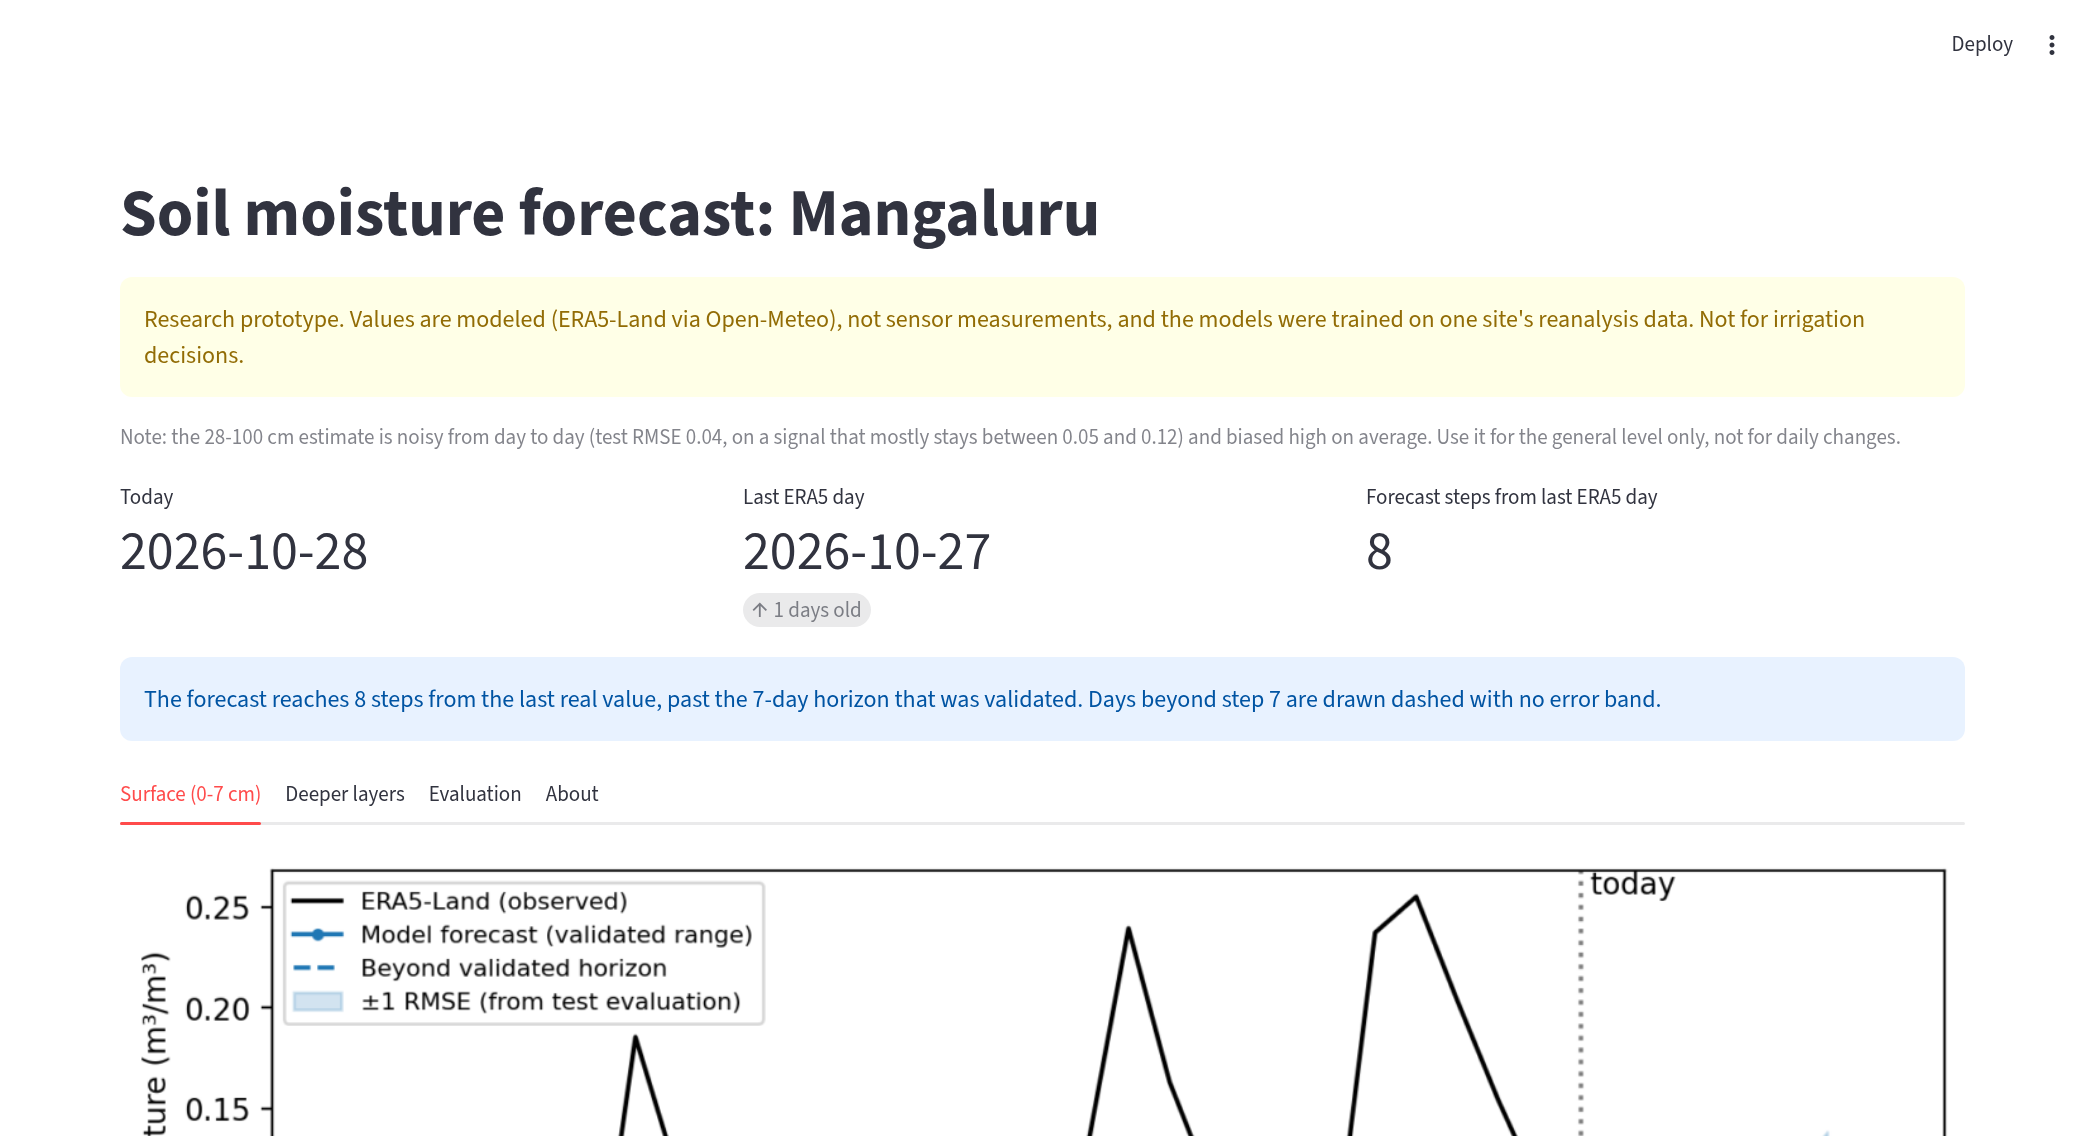
\includegraphics[width=\textwidth]{figures/dashboard_surface.png}\\
            \vspace{0.1cm}
            \footnotesize \textit{Live Surface (0--7 cm) forecast tab showing real-time metrics and chart.}
        \end{column}
    \end{columns}
\end{frame}

% ── Slide 15b: Dashboard Deep Layers & Evaluation Screenshots ────────
\begin{frame}{Dashboard: Deep Layer Tracking \& Model Evaluation}
    \begin{columns}
        \begin{column}{0.50\textwidth}
            \centering
            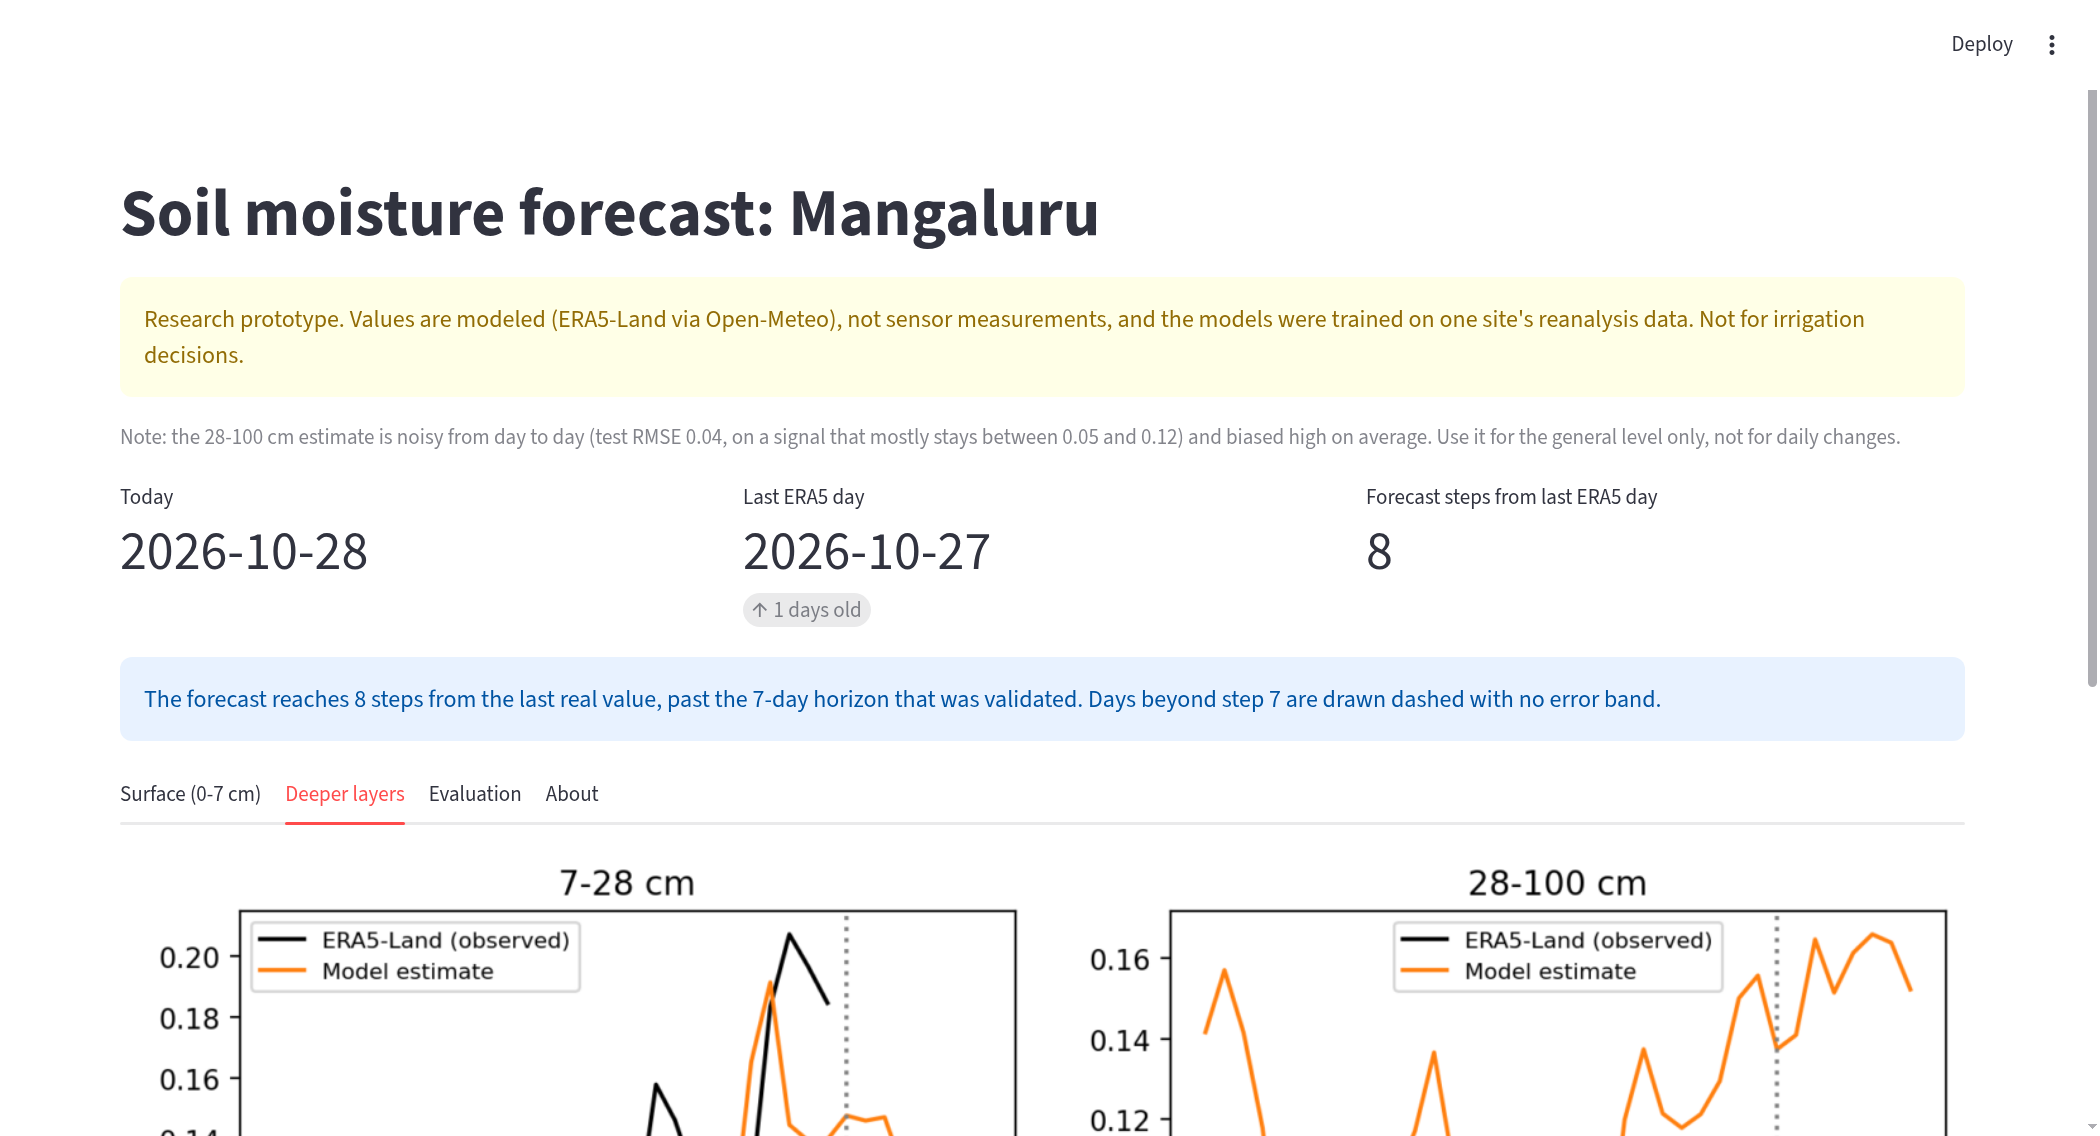
\includegraphics[width=\textwidth]{figures/dashboard_deep.png}\\
            \vspace{0.1cm}
            \footnotesize \textit{Deeper Layers tab: simultaneous 7--28 cm and 28--100 cm profile tracking.}
        \end{column}
        \begin{column}{0.48\textwidth}
            \centering
            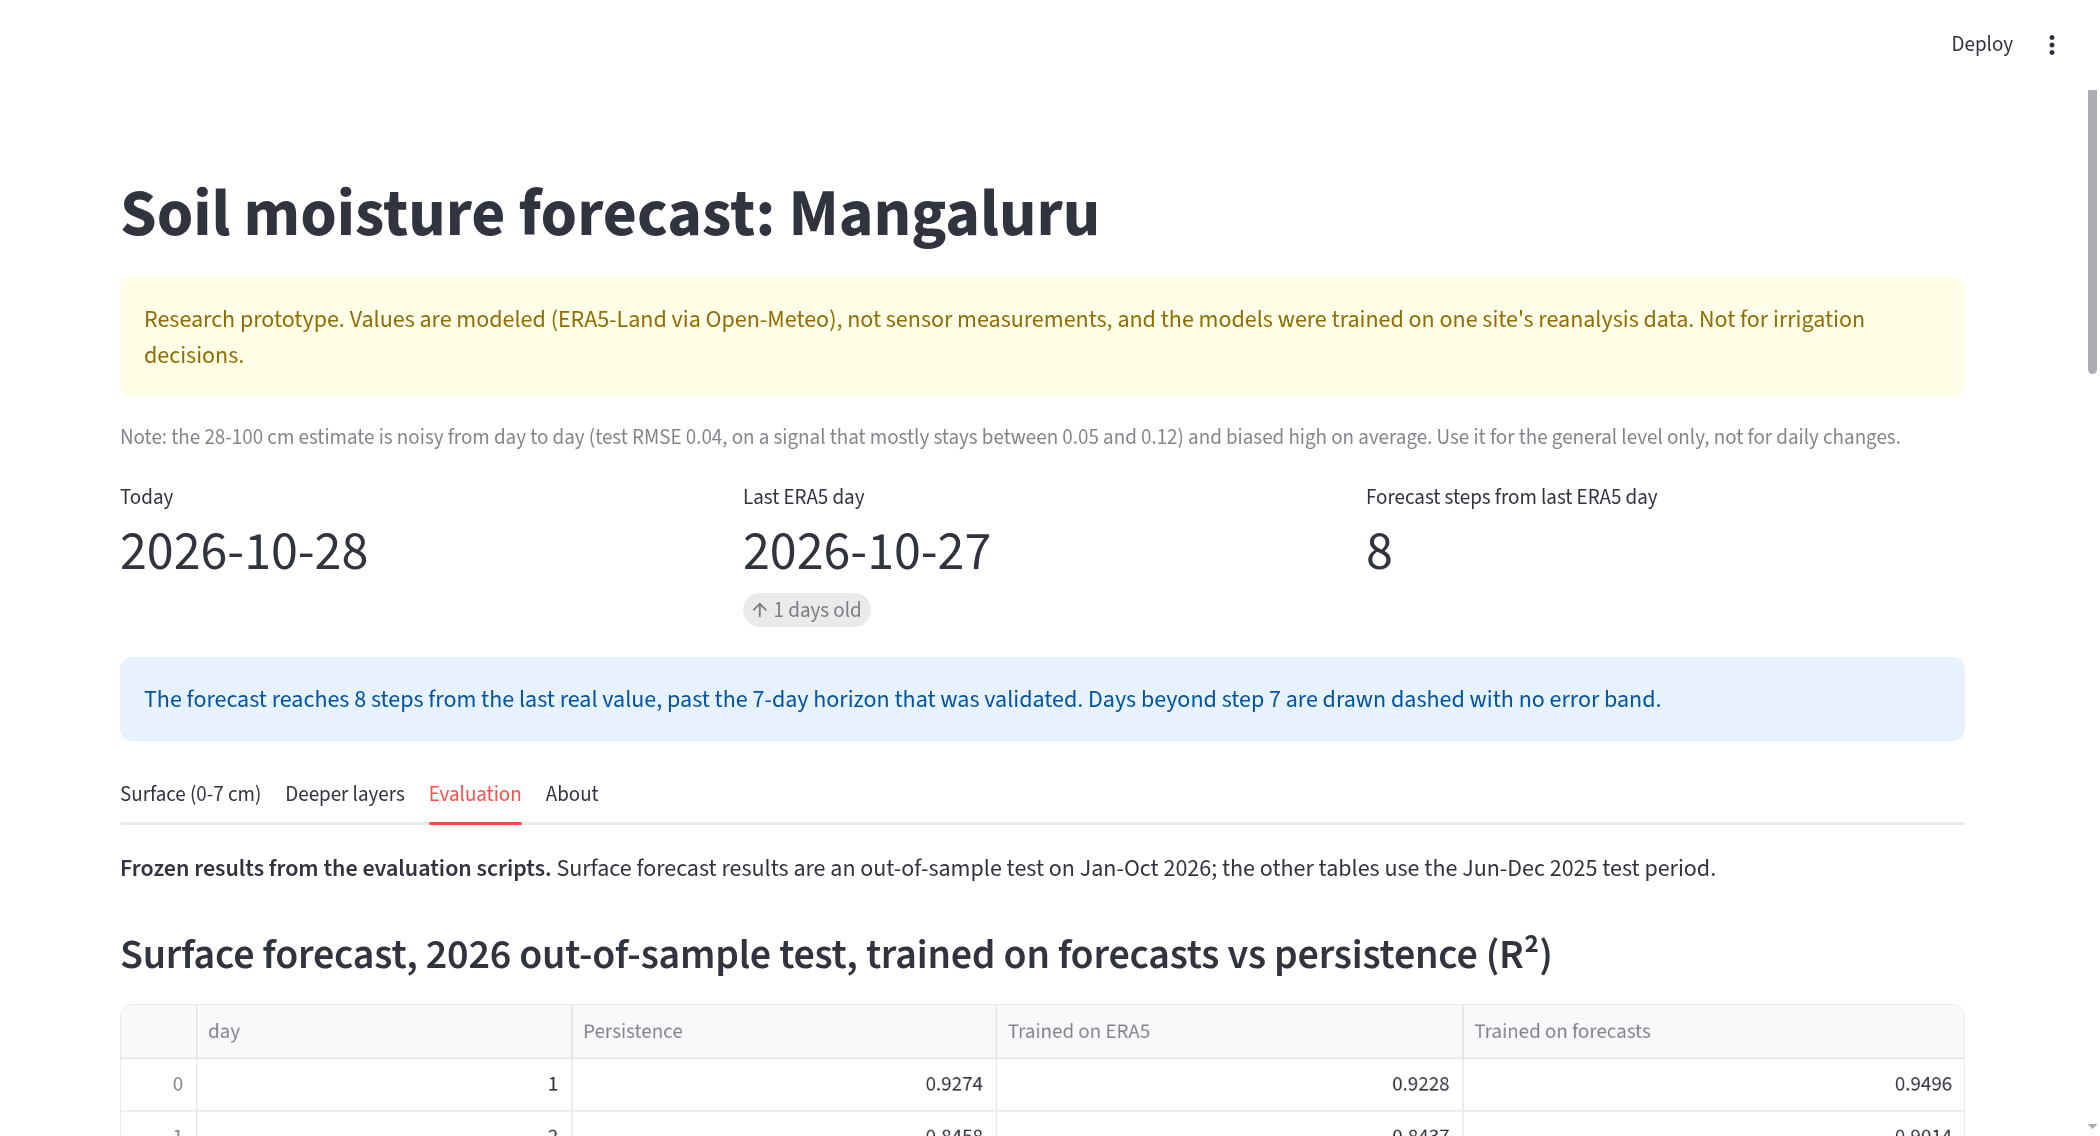
\includegraphics[width=\textwidth]{figures/dashboard_eval.png}\\
            \vspace{0.1cm}
            \footnotesize \textit{Evaluation tab: frozen R\textsuperscript{2} benchmarks across forecast methods.}
        \end{column}
    \end{columns}
\end{frame}

% ── Slide 16: Conclusions & Takeaways ─────────────────────────────────
\begin{frame}{Conclusions \& Practical Engineering Takeaways}
    \begin{columns}[t]
        \begin{column}{0.48\textwidth}
            \begin{block}{\textbf{Key Technical Achievements}}
                \footnotesize
                \begin{itemize}
                    \item Replicated and extended Gao et al.\ (2026) for tropical coastal Indian testbed (Mangaluru).
                    \item Proved that training on \textbf{real weather forecasts} preserves 7-day predictive power ($R^2 = 0.73$), preventing operational degradation.
                    \item Demonstrated that \textbf{long-memory feature engineering} unlocks accurate deep-layer estimation ($R^2 = 0.74\text{--}0.97$) without underground sensors.
                    \item Discovered that \textbf{SAR anomaly modeling} ($R^2 = 0.81$) is necessary to overcome tropical vegetation confounding.
                \end{itemize}
            \end{block}
        \end{column}
        \begin{column}{0.48\textwidth}
            \begin{exampleblock}{\textbf{Future Work \& Applications}}
                \footnotesize
                \begin{itemize}
                    \item \textbf{Spatial Transferability}: Expand pipeline across multiple agro-climatic zones with varying soil textures.
                    \item \textbf{In-Situ Ground Truthing}: Couple reanalysis predictions with physical in-field IoT soil sensor nodes.
                    \item \textbf{Deep Sequence Architectures}: Benchmark Temporal Convolutional Networks (TCN) or LSTMs for multi-horizon modeling.
                    \item \textbf{Smart Irrigation Automation}: Link profile moisture forecasts directly into crop evapotranspiration water-budget controllers.
                \end{itemize}
            \end{exampleblock}
        \end{column}
    \end{columns}
\end{frame}

% ── Slide 17: Thank You Slide ─────────────────────────────────────────
\begin{frame}[plain]
    \centering
    \vspace{1.0cm}
    {\Huge \textbf{\color{primaryblue}Thank You!}}\\[0.6cm]
    {\large \textbf{Questions \& Discussion}}\\[1.0cm]
    
    \begin{block}{\centering \textbf{Project Artifacts \& Source Code}}
        \centering
        \footnotesize
        \textbf{Repository}: Mangaluru Soil Moisture ML Pipeline\\
        \textbf{Report}: Comprehensive 25-page replication and extension study\\
        \textbf{Live Prototype}: Streamlit multi-depth interactive forecasting dashboard
    \end{block}
    
    \vspace{0.4cm}
    \footnotesize
    Department of Civil Engineering $\bullet$ National Institute of Technology Karnataka (NITK), Surathkal
\end{frame}

\end{document}
